%% Copernicus Publications Manuscript Preparation Template for LaTeX Submissions
%% ---------------------------------
%% This template should be used for copernicus.cls
%% The class file and some style files are bundled in the Copernicus Latex Package, which can be downloaded from the different journal webpages.
%% For further assistance please contact Copernicus Publications at: production@copernicus.org
%% http://publications.copernicus.org/for_authors/manuscript_preparation.html


%% Please use the following documentclass and journal abbreviations for discussion papers and final revised papers.


%% 2-column papers and discussion papers
\documentclass[acp, manuscript]{copernicus}

%% Journal abbreviations (please use the same for discussion papers and final revised papers)

% Archives Animal Breeding (aab)
% Atmospheric Chemistry and Physics (acp)
% Advances in Geosciences (adgeo)
% Advances in Statistical Climatology, Meteorology and Oceanography (ascmo)
% Annales Geophysicae (angeo)
% ASTRA Proceedings (ap)
% Atmospheric Measurement Techniques (amt)
% Advances in Radio Science (ars)
% Advances in Science and Research (asr)
% Biogeosciences (bg)
% Climate of the Past (cp)
% Drinking Water Engineering and Science (dwes)
% Earth System Dynamics (esd)
% Earth Surface Dynamics (esurf)
% Earth System Science Data (essd)
% Fossil Record (fr)
% Geographica Helvetica (gh)
% Geoscientific Instrumentation, Methods and Data Systems (gi)
% Geoscientific Model Development (gmd)
% Geothermal Energy Science (gtes)
% Hydrology and Earth System Sciences (hess)
% History of Geo- and Space Sciences (hgss)
% Journal of Sensors and Sensor Systems (jsss)
% Mechanical Sciences (ms)
% Natural Hazards and Earth System Sciences (nhess)
% Nonlinear Processes in Geophysics (npg)
% Ocean Science (os)
% Proceedings of the International Association of Hydrological Sciences (piahs)
% Primate Biology (pb)
% Scientific Drilling (sd)
% SOIL (soil)
% Solid Earth (se)
% The Cryosphere (tc)
% Web Ecology (we)
% Wind Energy Science (wes)

%% \usepackage commands included in the copernicus.cls:
%\usepackage[german, english]{babel}
%\usepackage{tabularx}
%\usepackage{cancel}
%\usepackage{multirow}
%\usepackage{supertabular}
%\usepackage{algorithmic}
%\usepackage{algorithm}
%\usepackage{amsthm}
%\usepackage{float}
%\usepackage{subfig}
%\usepackage{rotating}

\begin{document}

\title{Brominated VSLS and their influence on ozone under a changing climate}

% \Author[affil]{given_name}{surname}
\Author[1]{Stefanie}{Falk}
\Author[1]{Bj\"{o}rn-Martin}{Sinnhuber}
\Author[2]{Gis\`{e}le}{Krysztofiak}
\Author[3]{Patrick}{J\"{o}ckel}
\Author[3]{Phoebe}{Graf}
\Author[4]{Sinikka T.}{Lennartz}

\affil[1]{Institute of Meteorology and Climate Research, Karlsruhe Institute of Technology, Karlsruhe, Germany}
\affil[2]{LPC2E, Universit\'{e} d'Orl\'{e}ans, CNRS, UMR7328, Orl\'{e}ans, France}
\affil[3]{Deutsches Zentrum f\"{u}r Luft- und Raumfahrt e.V., Oberpfaffenhofen, Germany}
\affil[4]{Geomar, Helmholtz-Centre for Ocean Research Kiel, Kiel, Germany}
%% The [] brackets identify the author with the corresponding affiliation. 1, 2, 3, etc. should be inserted.

\runningtitle{Future change in brominated VSLS}

\runningauthor{Falk et al.}

\correspondence{Stefanie Falk (stefanie.falk@kit.edu)}

\received{}
\pubdiscuss{} %% only important for two-stage journals
\revised{}
\accepted{}
\published{}

%% These dates will be inserted by Copernicus Publications during the typesetting process.

\firstpage{1}

\maketitle

\begin{abstract}
Very short-lived source gases~(VSLS) contribute significantly to the tropospheric and stratospheric bromine loading. At present, an estimated 25\% of stratospheric bromine is of oceanic origin. In this study, we investigate how climate change may impact the ocean--atmosphere flux of brominated VSLS, their atmospheric transport, chemical transformations, and evaluate how these changes will affect stratospheric ozone over the 21st century.\\
Under the assumption of fixed ocean water concentrations and RCP6.0 scenario, we find an increase of the ocean--atmosphere flux of brominated VSLS of about 8--10\% by the end of the 21st century compared to present day.
A decrease in the tropospheric mixing ratios of VSLS and an increase in the lower stratosphere are attributed to changes in atmospheric chemistry and transport. Our model simulations reveal that, in line with the reduction in the troposphere, the total amount of bromine from VSLS in the stratosphere will decrease during the 21st century. Part of the apparent increase of VSLS in the tropical lower stratosphere results from an increase in the corresponding tropopause height. As the depletion of stratospheric ozone due to bromine depends also on the availability of chlorine, we find the impact of bromine on stratospheric ozone at the end of the 21st century reduced compared to present day.
Thus, these studies highlight the different factors influencing the role of brominated VSLS in a future climate.
\end{abstract}
%
%\clearpage
%
\introduction  %% \introduction[modified heading if necessary]
Ozone is an important trace gas in the Earth's atmosphere. The stratospheric layer of its highest abundance, the ozone layer, absorbs harmful ultraviolet~(UV) radiation threatening all lifeforms on the Earth's surface and acts as a potent greenhouse gas~(GHG). In the troposphere, ozone is considered a harmful pollutant. Catalytic cycles involving bromine and mixed halogen reactions, namely with chlorine, efficiently deplete ozone~\citep[e.g.,][]{ACP:Sinnhuber2009}. The ozone depletion efficiency of bromine is strongly related to the available amount of activated chlorine in the atmosphere~\citep{ACP:Yang2014,GRL:Sinnhuber2015,GRL:Oman2016}. Long-lived, anthropogenically emitted, halogenated source gases~(SG), e.g., \chem{CH_3Br} and Halons, have been restricted by the Montreal protocol and its amendments. Their atmospheric concentrations have started to decline globally~\citep[see][Chap. 1]{WMO2010}. Still, they contribute about 75\% to the overall bromine loading in the stratosphere. The remainder is provided by organic SG of oceanic origin of which methyl bromide (\chem{CH_3Br}), bromoform (\chem{CHBr_3}), and dibromomethane (\chem{CH_2Br_2}) are the most abundant. Minor brominated VSLS include the mixed bromo-chloro-carbons \chem{CHCl_2Br}, \chem{CHClBr_2}, and \chem{CH_2ClBr}. The tropospheric lifetime of these gases lies between several days to weeks, hence they are referred to as very short-lived source gases~(VSLS). They are produced by plankton and macroalgae, and are predominantly produced in coastal waters~\citep{JGR:Moore1996,LO:Lin2012,MC:Hughes2013,BGS:Stemmler2015}. Through gas exchange governed by the concentration gradient between ocean water ($c_\text{w}$) and atmosphere ($c_\text{w}$), solubility, and wind stress, VSLS are emitted into the atmosphere. Transport to the stratosphere, as shown by different model studies~\citep{ACP:Aschmann2009,GRL:Hossaini2012,ACP:Liang2014}, occurs in tropical regions of deep convection, most importantly the Western Pacific and Maritime Continent, in South East Asia, and over the Gulf of Mexico. Organic SG are transported through the tropical tropopause layer~(TTL) together with their inorganic product gases~(PG). PG are produced through photochemical decomposition of VSLS and provide reactive bromine (\chem{Br_y}, from \chem{Br}, \chem{Br_2}, \chem{HBr}, \chem{BrO}, \chem{BrONO_2}, \chem{BrNO_2}, \chem{BrCl}, and \chem{HOBr}) to the stratosphere. This is schematically shown in Fig.~\ref{fig:vsls_scheme}. In recent years, several approaches have been taken to describe the stratospheric or regional abundance of bromine from VSLS. Top-down scenarios~\citep{JGR:Warwick2006, ACP:Liang2010, ACP:Ordonez2012} match atmospheric observations by setting constant fluxes or boundary concentrations. Bottom-up scenarios~\citep[e.g.,][]{ACP:Ziska2013} developed emission climatologies by extrapolating measurements in the surface ocean and marine boundary layer and calculate emissions accordingly. As shown by \citet{ACP:Lennartz2015}, the bottom-up fluxes based on the oceanic water concentrations of \citet{ACP:Ziska2013} are in good agreement with available atmospheric VSLS observations.\\
In this study, we will address the open questions on how these oceanic emissions of VSLS evolve in response to a changing climate (Section~\ref{sec:emission_trends}), how transport and chemistry influence the stratospheric bromine abundance in a changing climate (Section~\ref{sec:bromine_loading}), and how ozone will be affected by the assumed changes in VSLS abundance (Section~\ref{sec:ozone_depletion}). Details about the model and simulations used in this study will be given in Section~\ref{sec:model_exp}.
%
\begin{figure}[t]
  \centering
  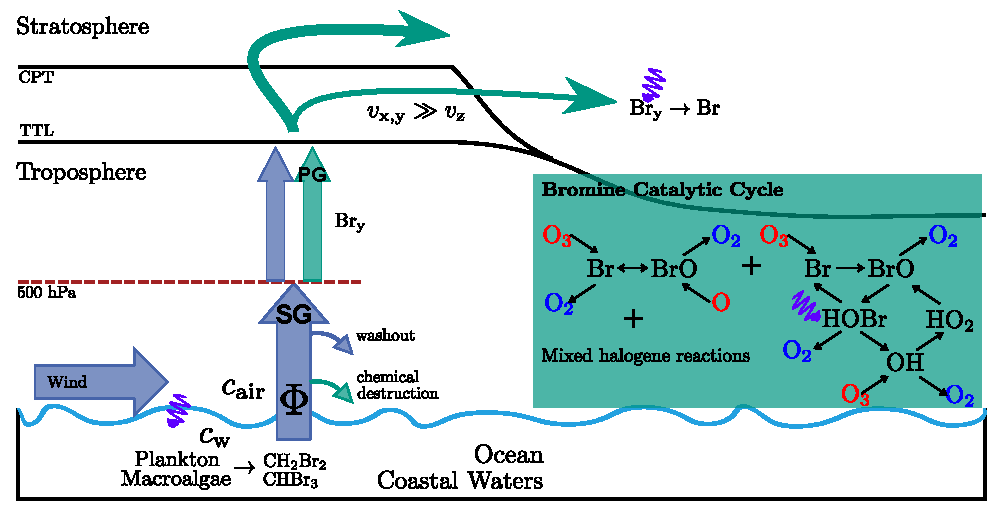
\includegraphics[width=8.3cm]{fig01}
  \caption{Scheme of VSLS emission and catalytic cycle of ozone depletion involving bromine.}
  \label{fig:vsls_scheme}
\end{figure}
%
\section{Model and experiments}
\label{sec:model_exp}
All model experiments have been performed using the ECHAM/MESSy Atmospheric Chemistry~(EMAC) model~\citep{GMD:Joeckel2010}. Table~\ref{tab:experiments} gives an overview over the key-factors of the simulations.\\
Future changes in fluxes of brominated VSLS from the ocean are studied with a free-running long-term simulation (SC\_free, 1979--2100) using a simplified chemistry (Section~\ref{sec:emission_trends}), augmented by a similar simulation, but nudged towards the European Centre for Medium-Range Weather Forecasts~(ECMWF) Re-Analysis (ERA)--Interim over the period 1979--2012. Therein, emission fluxes are computed online from prescribed sea water concentrations. The simplified-chemistry simulations use EMAC version 2.50 with submodels \texttt{airsea} \citep{ACP:Pozzer2006} ($k_\mathrm{w}$ parametrization~\citet{GRS:Nightingale2000}), \texttt{cloud}, \texttt{cloudopt}, \texttt{convect} (with operational ECMWF convection scheme), \texttt{cvtrans}, \texttt{ddep} \citep{ACP:Kerkweg2006b}, \texttt{ptracs} \citep{ACP:Joeckel2008}, \texttt{rad}, \texttt{scav} \citep{ACP:Tost2006}, \texttt{surface}, and \texttt{tnudge} \citep{ACP:Kerkweg2006} (set-up as in~\citet{ACP:Lennartz2015,ACP:Hossaini2016}). 
The tracer lifetime due to reaction with \chem{OH} has been fixed to monthly mean values from National Centre for Meteorological Research~(CNRM)~\citep{GMD:Michou2011,GMD:Morgenstern2016} model calculations, while photolysis rates are computed within the EMAC submodel \texttt{jval}~\citep{GMD:Sander2014}. In these simulations, \chem{OH} concentrations have been set to zero in the lower troposphere (700--1000\,\unit{hPa}) to reduce the variability of ground level volume mixing ratio~(VMR) of VSLS. Water concentrations of \chem{CH_2Br_2} and \chem{CHBr_3} have been held constant using the climatology of~\citet{ACP:Ziska2013}. For mixed bromo-chloro-carbons (\chem{CHBrCl_2}, \chem{CHBr_2Cl}, \chem{CH_2BrCl}), water concentrations have been estimated by scaling \chem{CHBr_3} concentrations to obtain a better agreement between model simulation and tropical mean profile and surface observations of these VSLS. Bromine produced by VSLS decomposition is commuted into \chem{Br_y}. The distribution into \chem{Br}, \chem{HBr}, \chem{BrO}, \chem{BrONO_2}, \chem{BrNO_2}, \chem{BrCl}, \chem{HOBr} in these simplified chemistry simulations has been computed offline from a full-chemistry EMAC simulation of one year duration with six hourly output. Scavenging is applied to \chem{Br}, \chem{Br_2}, \chem{HBr}, \chem{BrNO_2}, \chem{BrONO_2}, \chem{BrCl}, and \chem{HOBr}. Concentrations of \chem{CO_2}, \chem{CH_4}, \chem{CFC}, and \chem{N_2O} in SC\_free are taken from a CNRM CM5 model~\citep{CD:Voldoire2013} simulation with Representative Concentration Pathways~(RCP)~6.0 scenario~\citep{EJ:Fujino2006,GEE:Hijioka2008}.\\
%
Data of a full-chemistry long-term simulation~\citep[RC2-base-05,][]{GMD:Joeckel2016} over a time span of 150 years (1950--2100) and performed as part of a Chemistry-Climate Model Initiative~(CCMI) recommended set of simulations by the Earth System Chemistry-Climate Modelling~(ESCiMo) consortium will be used for studying changes in transport and partitioning of bromine species (Section~\ref{sec:bromine_loading}). In this simulation, VSLS fluxes have been held constant following scenario five of~\citet{JGR:Warwick2006}.\\
An intermediate-term experiment, consisting of a set of two simulations and spanning the years 2075--2100, has been performed for assessing implications on ozone depletion in a future climate with significantly lower chlorine loading in the atmosphere (Section~\ref{sec:ozone_depletion}). The simulations named RT1a and RT1b both include online computation of aerosol formation. Fluxes of \chem{CH_2Br_2} and \chem{CHBr_3} are computed online from sea water concentrations of~\citet{ACP:Ziska2013} using the EMAC submodel \texttt{airsea} (with the \citet{JGRC:Wanninkhof1992} $k_\mathrm{w}$ parametrization as in RC2-base-05) in case of RT1a. For assessing the impact of VSLS on ozone, all VSLS emissions have been switched off in RT1b.\\
The full-chemistry experiments use EMAC version 2.51 (RC2-base-05) and 2.52 (RT1a/b), respectively. The dynamics have not been specified except for a weak nudging of the equatorial wind quasi-biennial oscillation~(QBO). RC2-base-05 combines hindcast with future projections. The set-up of RT1a and RT1b is almost identical to RC2-base-05, thus we refer to the corresponding paper by the ESCiMo consortium~\citep{GMD:Joeckel2016} for general information. The major difference lies in the aforementioned treatment of VSLS emission, which is handled analogous to SC\_free, except for mixed bromo-chloro-carbons emissions taken from~\citet{JGR:Warwick2006}. Since heterogeneous reaction and chlorine activation are important for the depletion process of ozone, aerosol formation is computed online using the submodel \texttt{GMXe}~\citep{GMD:Pringle2010} of EMAC. The set-up has been adapted from RC1-aero-07~\citep{GMD:Joeckel2016} with modifications as in~\citet{ACP:Bruehl2012,JGR:Bruehl2015}. Radiation coupling had been activated in \texttt{GMXe}, but cloud coupling had not been activated. In this regard, an additional oceanic sulfur source, carbonyl sulfide (COS), which is a major source of stratospheric sulfur has been included in addition to dimethyl sulfide (DMS). Whereas the emission of the latter is computed from prescribed ocean concentrations, constant fluxes of COS have been adopted from~\citet{JGR:Kettle2002}. Additional reaction pathways of sulfur have been enabled accordingly. RT1a and RT1b have been initialized with available monthly mean values from RC2-base-05. COS has been initialized from a simulation which results have been published recently~\citep{GRL:Glatthor2015}, including an artificially increased oceanic source to close the atmospheric budget.\\
The model's spatial resolution is T42L39MA for the simplified chemistry experiments, T42L47MA for RC2-base-05 respectively T42L90MA for RT1a/RT1b, corresponding to a $2.8^\circ\times 2.8^\circ$ grid, with a top level at 0.01\,\unit{hPa}. Emissions of GHG follow the RCP6.0 scenario and sea surface temperature~(SST) and sea ice cover~(SIC) are prescribed from Hadley Centre Global Environment Model version 2~(HadGEM2) forced with the RCP6.0 scenario for all simulations accordingly.
%
\begin{table*}[t]
  \centering
  \caption[]{EMAC model experiments used in this study. All experiments follow the RCP6.0 scenario of GHG emissions and have accordingly prescribed SST and SIC from HadGEM2.}
  \begin{tabular}{lcccccc}
    \tophline
    Experiment & Model Version & Resolution & Time-Span & Chemistry & VSLS Emission & Interactive Aerosols\\
    \middlehline
    SC\_nudged & 2.50 & T42L39MA & 1979--2012 & simplified bromine & \texttt{airsea} & no\\
    SC\_free & 2.50 & T42L39MA & 1979--2100 & simplified bromine & \texttt{airsea} & no\\
    RC2-base-05 & 2.51 & T42L47MA & 1950--2100 & full & \citet{JGR:Warwick2006} & no\\
    RT1a & 2.52 & T42L90MA & 2075--2100 & full + sulfur & \texttt{airsea} & yes\\
    RT1b & 2.52 & T42L90MA & 2075--2100 & full + sulfur & none & yes\\
    \bottomhline
  \end{tabular}
  \label{tab:experiments}
\end{table*}
\section{Long-term Trends in Oceanic Emission Fluxes}
\label{sec:emission_trends}
In this section, we investigate how a changing climate may influence emission fluxes of VSLS from the ocean. We will assess the impact of changing physical factors (e.g., SST, SIC, and wind speed) on ocean--atmosphere gas exchange driven by the RCP6.0 scenario. Here we assume constant oceanic concentrations of VSLS over the course of the century (following~\citet{ACP:Ziska2013,ACP:Lennartz2015}). This specific assumption might not hold since the effects of climate change, e.g., increase of ocean temperature, acidification, change of salinity, and nutrient input, on marine organisms and thus the production of \chem{CH_2Br_2} and \chem{CHBr_3} is not yet fully understood. Recent combined marine ecosystem model studies imply a global decrease of net primary production~(NPP) by plankton over the course of the 21st century~\citep{BGS:Laufkoetter2015,BGS:Laufkoetter2016}. However, the impact on bromocarbon concentration, predominantly produced by macroalgae in coastal regions, remains unclear.\\
%
As implemented in the EMAC submodel \texttt{airsea}~\citep{ACP:Pozzer2006}, the flux of a gas dissolved in ocean water to the atmosphere is governed by its concentration gradient $\Delta c$ and transfer velocity $k$, 
\begin{align}
  \label{eq:airsea}
  \Phi &= k \cdot \Delta c \\ \notag
       &= k\cdot \left(c_\text{w} - H\cdot c_\text{air}\right),
\end{align}
with $k = \left(1/k_\mathrm{w}+R\cdot H \cdot T_\mathrm{air}/k_\mathrm{air}\right)^{-1}$, wherein, $R$ is the universal gas constant and $H$ is the Henry coefficient for a specific gas. The transfer velocity depends largely on temperature $T$ and surface wind speed. The corresponding water and atmospheric concentrations are named $c_\mathrm{w}$ and $c_\mathrm{air}$.\\ 
In Fig.~\ref{fig:timeseries_integrated_seasonal_flux}, the difference of VSLS fluxes with respect to the start of the simulation in 1979 is shown for the free-running and nudged simplified-chemistry simulation. For both, \chem{CH_2Br_2} and \chem{CHBr_3}, all zonal bands display linearly rising fluxes. The strongest increase with respect to 1979 values is found in the tropical zone (20$^\circ$~N--20$^\circ$~S) with roughly 2.5\,\unit{\mathrm{Gg\,yr^{-1}}} and 13\,\unit{\mathrm{Gg\,yr^{-1}}} for \chem{CHBr_3} and \chem{CH_2Br_2} respectively. Relative to the absolute zonal fluxes, this yields an increase of about 10\% over the course of the century (Table~\ref{tab:relative_flux_increase}). The increase is slightly stronger in the southern tropics. The strongest relative increase in flux is found in the northern hemisphere polar region (90$^\circ$~N--50$^\circ$~N), with 25\% and roughly 55\% for \chem{CHBr_3} and \chem{CH_2Br_2}, respectively.\\
%
\begin{table*}[t]
  \centering
  \caption[]{Average absolute flux in 2000 in \unit{\mathrm{Gg\,yr^{-1}}} and percentage of relative increase in VSLS flux between 2000 and 2100 from SC\_free. The numbers have been obtained by linear regression of the data shown in Fig.~\ref{fig:timeseries_integrated_seasonal_flux} and evaluated at the given years.}
  \begin{tabular}{r@{--}l  r@{.}l r@{.}l r@{.}l r@{.}l}
    \tophline
     \multicolumn{2}{c}{Region} & 
     \multicolumn{4}{c}{\chem{CH_2Br_2}} & 
     \multicolumn{4}{c}{\chem{CHBr_3}}\\
     \multicolumn{2}{c}{} &
     \multicolumn{2}{l}{(\unit{\mathrm{Gg\,yr^{-1}}})} &  \multicolumn{2}{l}{(\%)} &
     \multicolumn{2}{l}{(\unit{\mathrm{Gg\,yr^{-1}}})} &  \multicolumn{2}{l}{(\%)}\\
     \middlehline
     $\mathrm{90^\circ N}$ & $\mathrm{50^\circ N}$ & 0&6 & 54&6 & 23&5  & 25&0\\
     $\mathrm{50^\circ N}$ & $\mathrm{20^\circ N}$ & 8&2 & 14&6 & 41&7  & 8&7\\
     $\mathrm{20^\circ N}$ & $\mathrm{0}$ & 19&2 & 6&6 & 52&4  & 8&6\\
     $\mathrm{0}$ & $\mathrm{20^\circ S}$ & 5&5 & 11&9 & 44&4  & 10&0\\
     $\mathrm{20^\circ S}$ & $\mathrm{50^\circ S}$ & 4&3 & 18&0 & 33&2  & 8&2\\
     $\mathrm{50^\circ S}$ & $\mathrm{90^\circ S}$ & 6&9 & 6&8 & 12&7  & 8&9\\
     \bottomhline
  \end{tabular}
  \label{tab:relative_flux_increase} 
\end{table*}
%
Regarding the changing physical factors, the HadGEM2 prescribed SSTs are increasing almost linearly over the course of the century (Fig.~\ref{fig:hadgem2_input}a). Under the RCP6.0 scenario, this increase in SST ranges between 1\,\unit{^\circ\,C}--3.5\,\unit{^\circ\,C}. The weak rise in Antarctic SST is accompanied by a weakly increasing Antarctic flux of VSLS. The corresponding HadGEM2 prognosticated retreat of Arctic sea ice is shown in Fig.~\ref{fig:hadgem2_input}b. Sea ice is not regarded as a source of VSLS in our study and therefore only acts as a lid blocking the ocean to atmosphere flux. Hence, a polar sea which is to a large extent free of sea ice will have increased fluxes of VSLS. In accordance, the Arctic August--September maximum of flux is expected to be more pronounced. 
%Zonally averaged seasonal cycles of fluxes are shown in Fig.~\ref{fig:integrated_seasonal_flux} for both VSLS species. Solid lines herein refer to a present day average (1990--2000) and dashed lines to future (2090--2100). 
Distinct maxima in the seasonal cycles are found for summer months on both hemispheres and minima occurring in late winter. There is a slightly stronger increase of fluxes in the future during the time periods of maxima, but no change in phase. In case of \chem{CH_2Br_2}, even negative emissions are found during winter at high-latitudes on the northern hemisphere. In the northern tropics, \chem{CHBr_3} shows a distinct maximum in northern hemisphere summer, while the southern tropics do not display any seasonal cycle. Albeit increased ocean--atmosphere fluxes in the future, only taking the changes of physical factors into account, seasonal cycles remain largely the same. In our simulations, zonally averaged absolute wind speed at 10\,\unit{m} is only slightly changing over the course of the 21st century (-4--2\%). Thus, it is indicated by our simulations, that the important factor regarding an increase of ocean--atmosphere flux of VSLS is the change in SSTs.\\
%
In Fig.~\ref{fig:gisele-vsls-profiles}, resulting VMR profiles of organic (\chem{Br_{org}}) and inorganic bromine (\chem{Br_y}) from VSLS are shown. VSLS data have been averaged over a time period 1990--2000 and 2090--2100. The VMR profile of \chem{Br_{org}} displays a steep decline in the lower troposphere (400--1000\,\unit{hPa}) by more than 50\% of ground level VMR, stays almost constant before entering the stratosphere, where VSLS are quickly dissociated. Comparing present day and future values (keeping in mind that \chem{OH} concentration are nudged towards monthly mean values of \chem{OH} and photolysis rates are fixed in SC\_free), \chem{Br_{org}} is found to have increased through out the atmosphere by about 0.1--0.4\,\unit{ppt}. In the lower stratosphere, this increase amounts to about 0.3\,\unit{ppt} (8\%). VMR of \chem{Br_y} is increased from the lower stratosphere upwards by roughly 0.4\,\unit{ppt} (10\%). These changes in the vertical profiles can be attributed to enhanced emissions in a future climate which, as shown, are of the order of 10\%.\\
%
As can be inferred from Eq.~(\ref{eq:airsea}), ocean--atmosphere fluxes are sensitive to the abundance of VSLS in the atmosphere as well as a differing wind speed parametrization. An increased chemical dissociation of VSLS in the lowermost troposphere (e.g., due to a probable future increase in \chem{OH}) would reduce the atmospheric concentration and therefore increase the flux from the ocean to the atmosphere without increasing the actual amount which is transported to the stratosphere. In this regard, fluxes from RT1a have been compared to SC\_free in 2100. Much stronger fluxes (1.3--1.5 times) have been found in the former simulation in comparison to the latter. Underlying changes in photochemical dissociation and tracer transport due to a changing climate have not been disentangled at this point and will be studied in detail in the following section.
%
\begin{figure}[t]
  \centering
  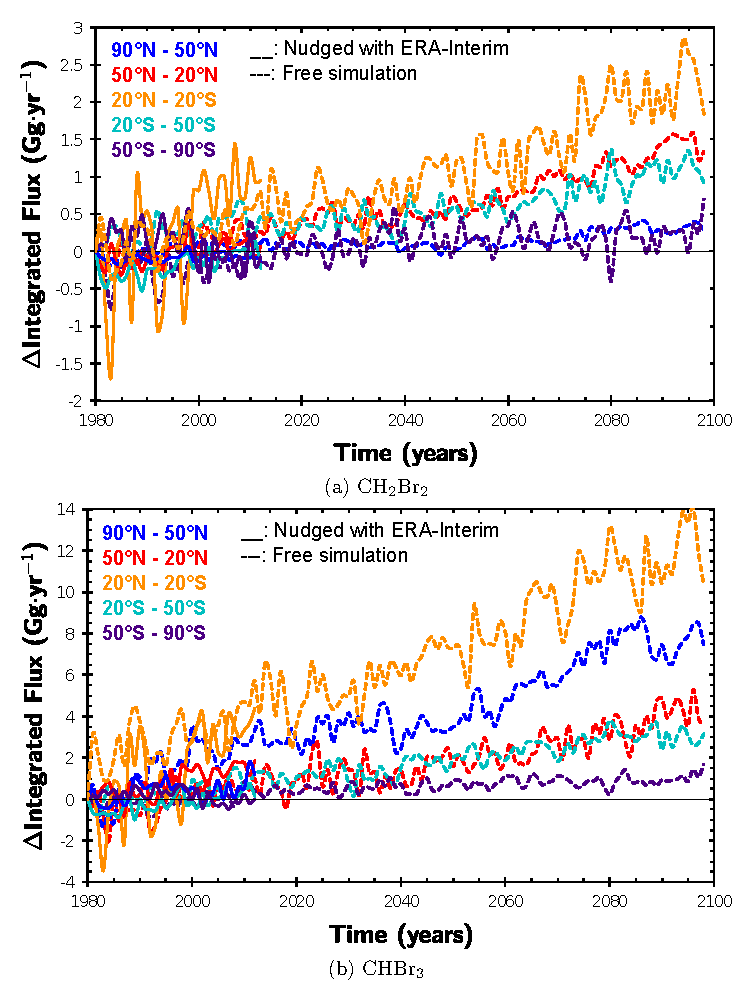
\includegraphics[width=8.3cm]{fig02}
  \caption[]{Difference of integrated flux separated in different zonal bands. Simplified chemistry EMAC simulation (SC\_free and SC\_nudged) with \texttt{airsea} gas exchange, water concentrations held constant. Solid lines represent ERA--Interim nudged (1979--2012) and dashed lines free-running (1979--2100).}
  \label{fig:timeseries_integrated_seasonal_flux}
\end{figure}
%
\begin{figure}[t]
  \centering
  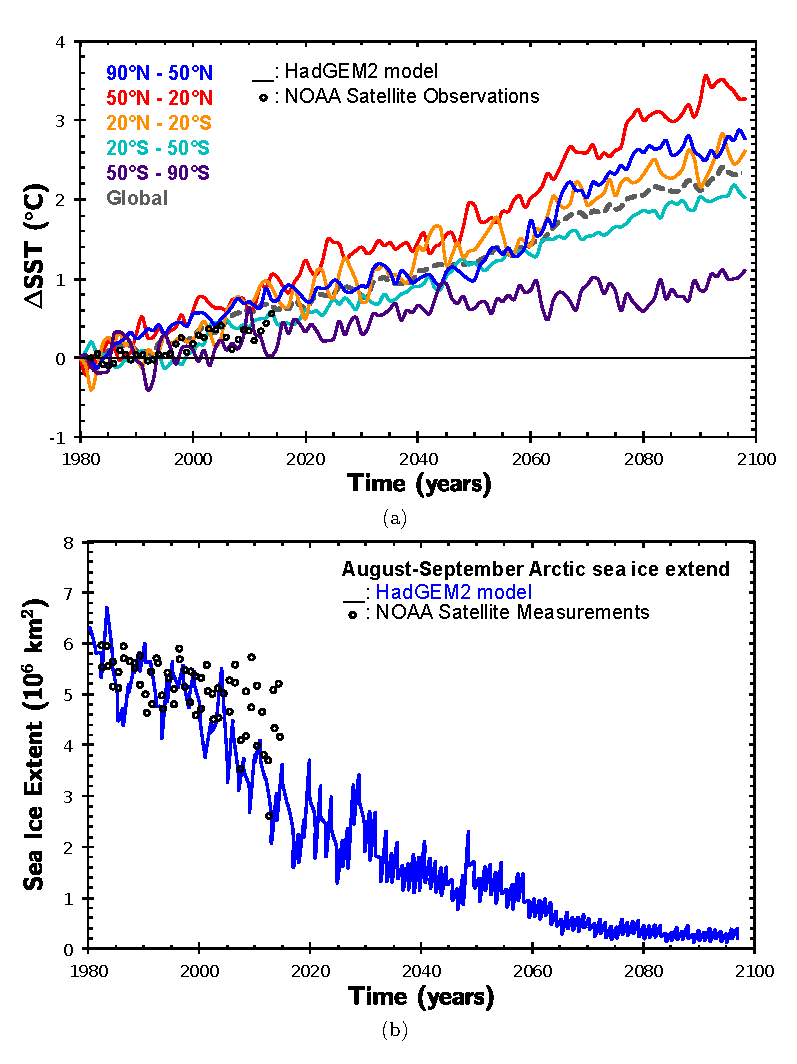
\includegraphics[width=8.3cm]{fig03}
  \caption[]{HadGEM2 prescribed ocean properties in the simplified-chemistry simulations compared to National Oceanic and NOAA Optimum Interpolation~(OI)~V2 fields~\citep{JC:Reynolds2002}. (a) Change in sea surface temperature for different latitude bands. Global average is shown as dashed gray line. (b) Arctic sea ice extend in August and September.}
  \label{fig:hadgem2_input}
\end{figure}
%
%\begin{figure}[t]
%  \centering
%  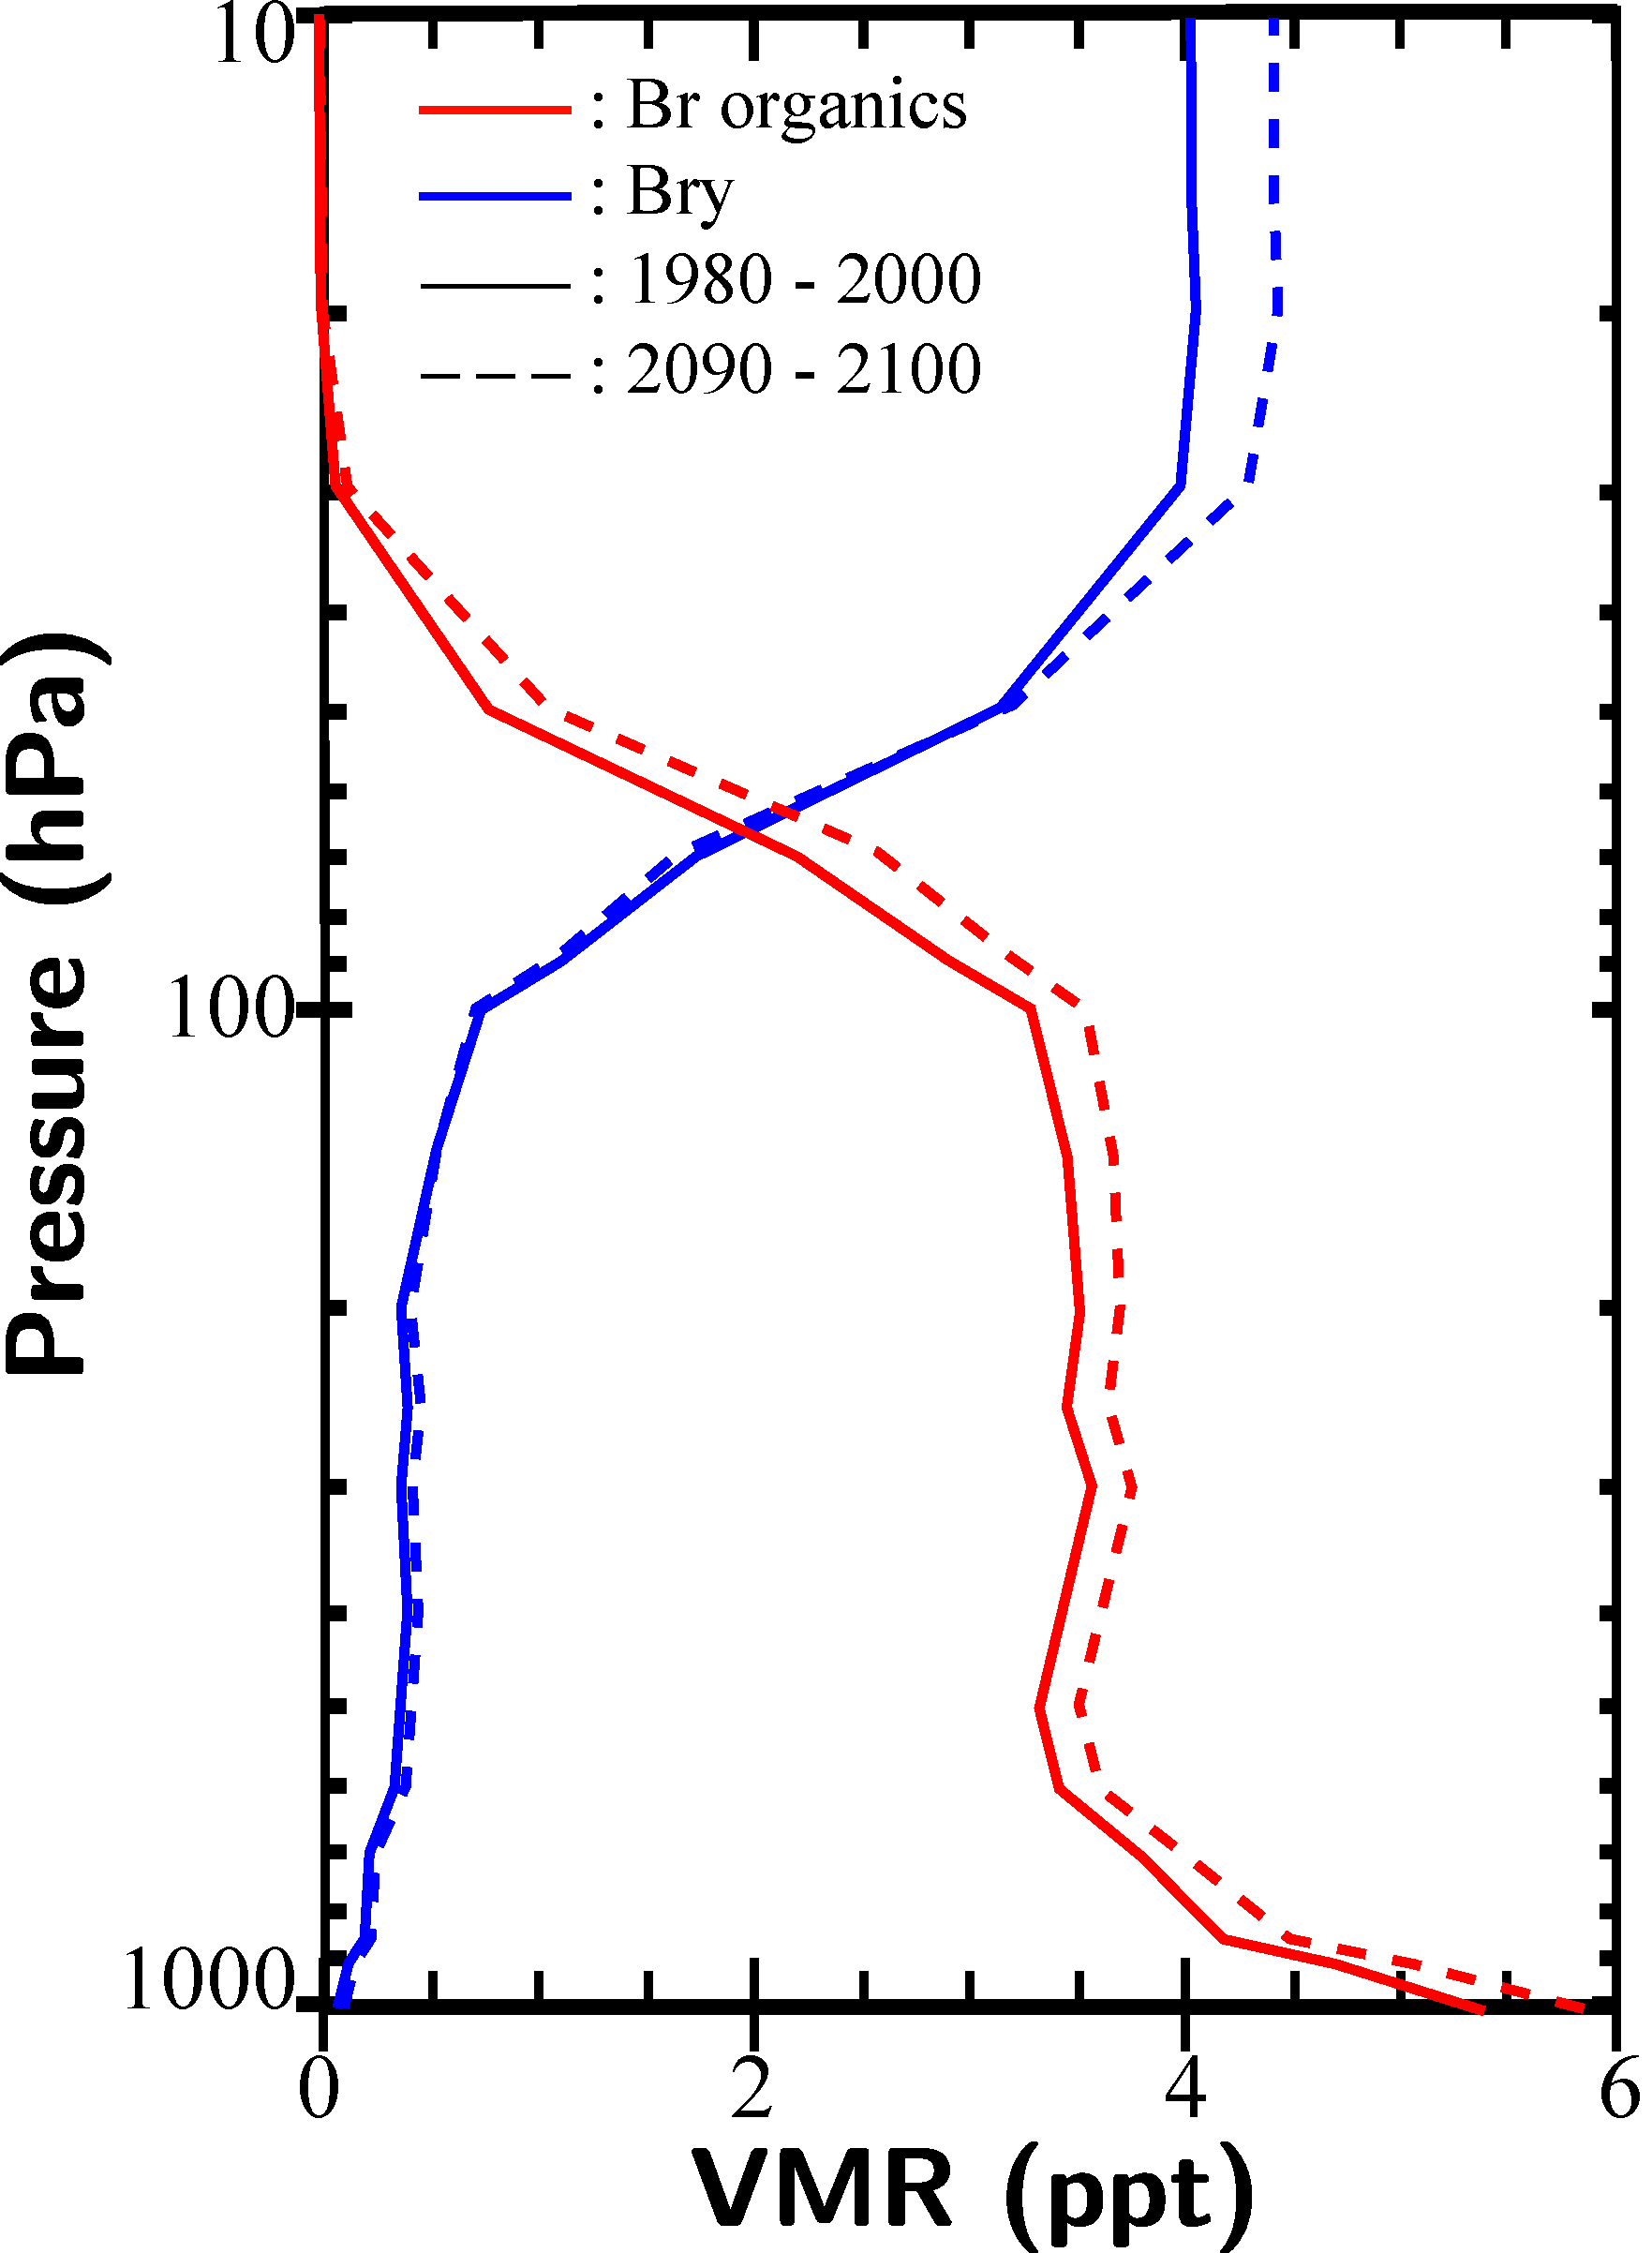
\includegraphics[width=8.3cm]{fig04}
%  \caption[]{Seasonal variation of integrated VSLS fluxes from EMAC simplified-chemistry simulation (1979--2100). 10 year averaged zonal means are shown with standard error on mean as shaded error bands. Solid lines refer to present-day mean (1990--2000) and dashed lines to future mean (2090--2100)}
%  \label{fig:integrated_seasonal_flux}
%\end{figure}
%
\begin{figure}[t]
  \centering
  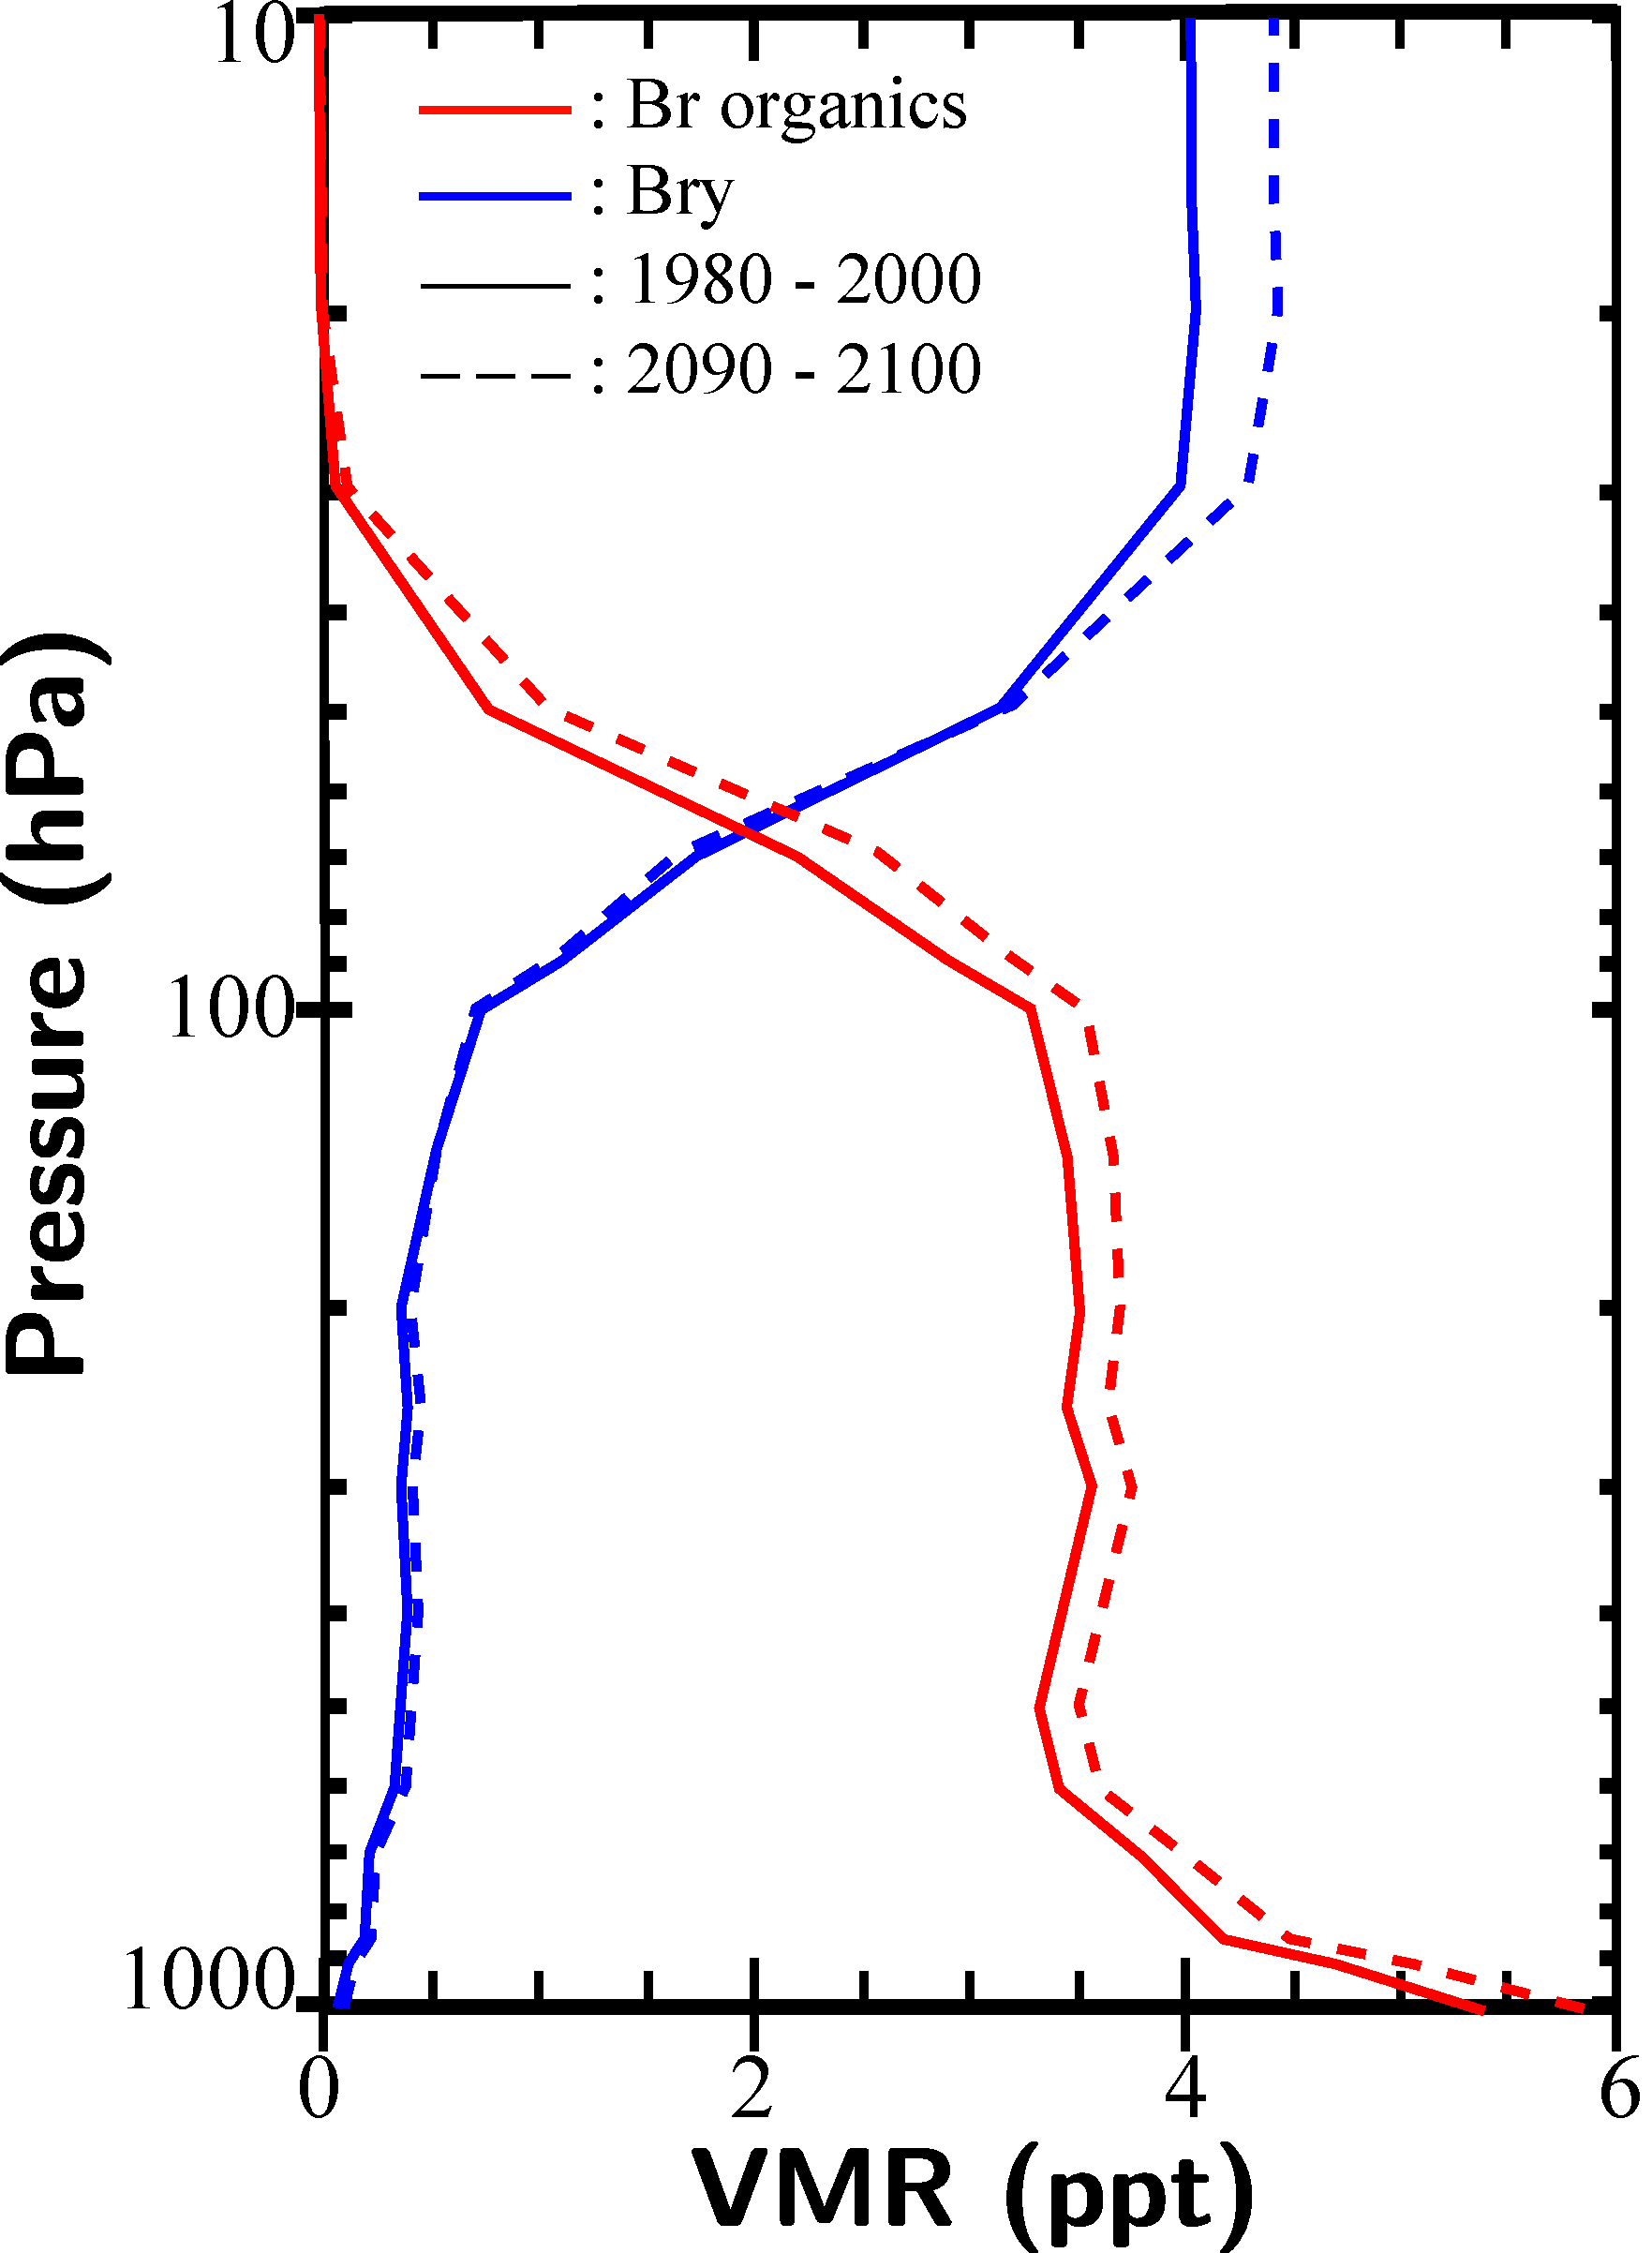
\includegraphics[width=8.3cm]{fig04}
  \caption[]{Tropical zonal mean (20$^\circ$~N--20$^\circ$~S), temporally averaged, vertical profiles of organic (\chem{Br_{org}}) and inorganic bromine (\chem{Br_y}) for the time periods 1990--2000 and 2090--2100 from SC\_free. In consistency with increasing VSLS fluxes (10\%), an increase of roughly 10\% in \chem{Br_y} from VSLS in the stratosphere is found, while the increase in \chem{Br_{org}} amounts to 8\%.}
  \label{fig:gisele-vsls-profiles}
\end{figure}
%
\section{Stratospheric bromine loading}
\label{sec:bromine_loading}
In addition to the possible increase in oceanic VSLS emissions due to climate change, discussed in the previous section, atmospheric transport and chemical transformation processes are also sensitive to climate change and may contribute to a change in the future stratospheric bromine loading from VSLS. These aspects will be studied in this section, based on the RC2-base-05 ESCiMo simulation, spanning 150 years from 1950 to 2100, assuming constant VSLS fluxes. Hence the fluxes of VSLS do not response to changes in the ground level abundances of VSLS.\\
%
In Fig.~\ref{fig:annual_mean_change_vsls}, profiles of brominated substances are shown for the tropics. The profiles are weighted by the amount of bromine atoms per molecule. The whole 150 year data set has been smoothed using a moving average with a box window size of 11 years to account for, e.g., seasonal variations, and the solar cycle. From these smoothed data, three reference years have been chosen for the analysis: 1980, 2016, and 2100. Therefore, 2100 is referring to June of the last valid year of the smoothed data (2094). To guide the eye, the corresponding mean tropical tropopause heights from the model output are shown together with the profiles. There is an upward shift of the tropopause height of about 8\,\unit{hPa} between present day and future. An upward shift of VSLS VMR profiles in 2100 in comparison to past/present day profiles is also visible. In the RCP6.0 scenario, ground level VMR of \chem{CH_3Br} and VSLS are constant from 2016 onward. In case of \chem{CH_3Br}, this roughly amounts to 1980 values. For all years, we find a fast decrease of VSLS of 5\,\unit{ppt} with a standard deviation of 0.25\,\unit{hPa} (or about 50\% compared to ground level VMR) between the surface and the mid-troposphere at about 500\,\unit{hPa}. The comparison of the difference of profiles between future and past/present (Fig.~\ref{fig:annual_mean_change_vsls}a, lower panel) reveals decreasing bromine values from VSLS by about 0.1--0.8\,\unit{ppt} throughout the troposphere, while there is an increase of the same order of magnitude in the lower stratosphere. Similar results have been published for RCP4.5 and RCP8.5 scenarios, attributing these to changes in the tropospheric circulation and to the primary oxidant \chem{OH}~\citep{GRL:Hossaini2012}. PG from VSLS (\chem{Br_y^{VSLS}}), which have been traced within the simulation, are decreasing in the stratosphere in the future. For 2016, this decline is compatible with a decreasing amount of VSLS in the troposphere. A slight excess of \chem{Br_y^{VSLS}} compared to 2016 and 2100 is found for 1980 in the stratosphere. This excess and the strong variability (denoted by the shown standard deviation) can be attributed to the hindcast period (1950--2005) of the simulation including volcanic eruptions. Large volcanic eruptions can influence the transport of bromine from VSLS into the stratosphere which may be related to a similar effect as seen in stratospheric water vapor~\citep{ACP:Loeffler2016}. Since volcanic activity has not been included in the future scenario, there is no such impact on \chem{Br_y^{VSLS}} from 2005 onward.\\
%
The largest change between present and future stems from the estimated decrease of long-lived SG, in particular Halons and \chem{CH_3Br}. At present, Halons contribute about 6--7\,\unit{ppt} to the total bromine loading of the lower stratosphere ($\sim$23\,\unit{ppt}), which is about the same amount as VSLS and \chem{CH_3Br} in RC2-base-05, whereas by the end of the century their contribution is reduced significantly to 1--2\,\unit{ppt} of total bromine ($\sim$17\,\unit{ppt}). This decline in long-lived, anthropogenically emitted SG is altering the amount of bromine released in the stratosphere on longer time scales. VSLS are already reduced due to photochemical dissociation when entering the TTL, while Halons are dissociating more slowly, providing a long lasting source of bromine to the stratosphere (Fig.~\ref{fig:annual_mean_change_vsls}b, lower panel). It is important to note, that although there is an apparent increase of \chem{Br_{org}^{VSLS}} of 0.5\,\unit{ppt} in the stratosphere assuming constant ocean--atmosphere fluxes, the overall amount of bromine in the stratosphere due to VSLS is decreasing in the future.\\
%
In the following, we will derive a semi-analytic model to separate various aspects affecting the future VSLS distribution in the atmosphere (Section~\ref{subsec:local_lifetime}). Since the atmospheric window for air entering the stratosphere is located in the tropics, we will focus on averaged tropical atmospheric quantities. Subsequently, the transition between troposphere and stratosphere caused by a rising tropopause is influencing the interpretation of VMR profile differences between present and future. This will be discussed in Section~\ref{subsec:tropopause}.
%
\begin{figure*}[t]
  \centering
  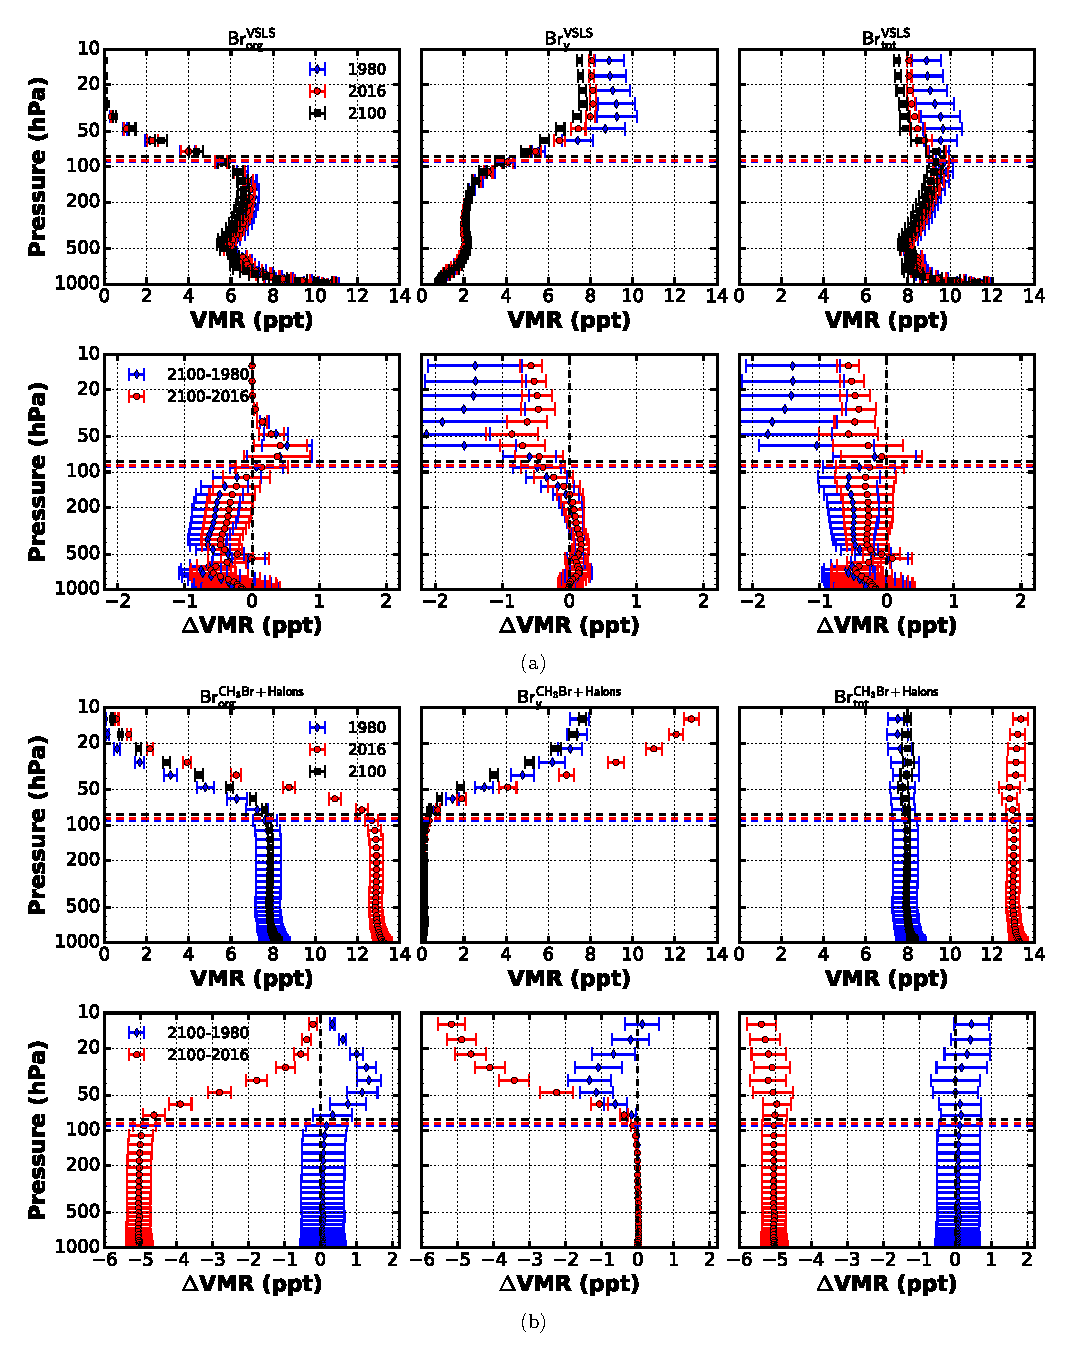
\includegraphics[width=12cm]{fig05} 
  \caption[]{Vertical profiles of brominated substances divided into SG (\chem{Br_{org}}), PG (\chem{Br_y}), and SG + PG (\chem{Br_{tot}}) in the tropics (20$^\circ$~N--20$^\circ$~S). Data from ESCiMo RC2-base-05 simulation~\citep{GMD:Joeckel2016}. Absolute values upper line, difference with respect to 2100 values bottom line. (a) Bromine from VSLS; (b) Bromine from \chem{CH_3Br} and Halons.}
  \label{fig:annual_mean_change_vsls}
\end{figure*}
%
%\begin{figure*}[t]
%  \centering
%  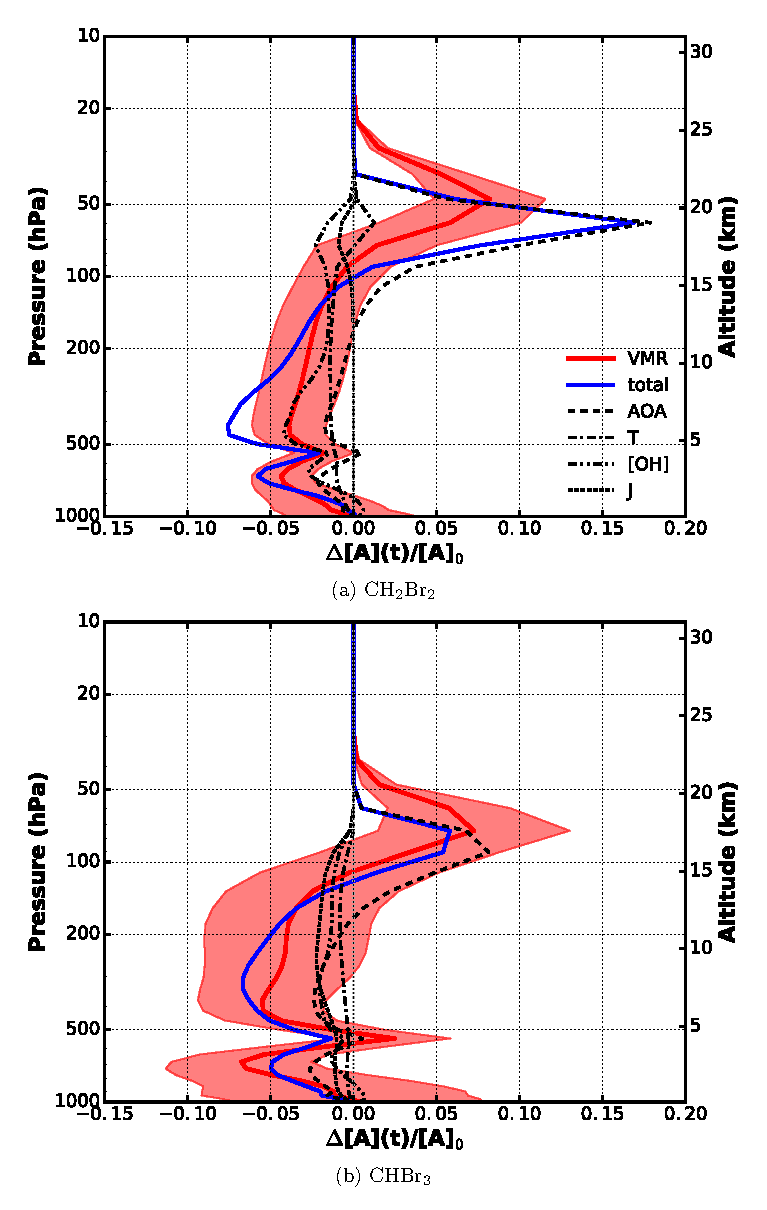
\includegraphics[width=12cm]{fig07}
%  \caption[]{VMR profiles of bromine from organic brominated source gases and total of bromine from inorganic product gases for past (1980), present (2016), and future (2100). Species have been scaled according to their amount of bromine.}
%  \label{fig:rc2-base-05-all_profiles}
%\end{figure*}
%
\subsection{Quantification of future atmospheric changes affecting VSLS mixing ratio profiles}
\label{subsec:local_lifetime}
The increase of VSLS in the stratosphere in the future can be attributed to changes in chemical and photolytical dissociation rates, and alternating transport from source regions through the TTL caused by a speed-up of the Brewer--Dobson circulation~(BDC).  
All of these factors influence the lifetime of VSLS in the atmosphere. A volume of air in a certain height (or rather pressure coordinate) shall have an associated mean temperature $T$, \chem{OH} concentration [\chem{OH}], photolysis frequency $J$, and age of air~(AOA). 
In the model, VSLS are dissociated photochemically via
%
\begin{reaction}
  \label{reac:oxi_CH2Br2}
  \chem{CH_2Br_2} + \chem{OH} \rightarrow \chem{2Br} + \chem{H_2O},
\end{reaction}
%
\begin{reaction}
  \label{reac:oxi_CHBr3}
  \chem{CHBr_3} + \chem{OH} \rightarrow \chem{3Br} + \chem{H_2O},
\end{reaction}
and 
\begin{reaction}
  \label{reac:photo_CH2Br2}
  \chem{CH_2Br_2} + h\nu \rightarrow \chem{2Br} + \chem{products},
\end{reaction}
%
\begin{reaction}
  \label{reac:photo_CHBr3}
  \chem{CHBr_3} + h\nu \rightarrow \chem{3Br} + \chem{products}.
\end{reaction}
The simplification in these equations compared to reality is justified since the intermediate reaction products \chem{CBr_2O} and \chem{CHBrO} insignificantly amount to the total bromine PG~\citep{ACP:Hossaini2010}.
From the resulting first order differential equation
%
\begin{equation}
  \label{eq:kin_gas}
  \frac{\mathrm{d[A]}}{\mathrm{d} t} = -k_\mathrm{A}(T)\cdot [\chem{OH}]\cdot \mathrm{[A]} - J_\mathrm{A} \cdot \mathrm{[A]},
\end{equation}
%
with [A] any of the VSLS species concentration, $k_\mathrm{A}(T)$ the temperature dependent rate coefficient, $J_\mathrm{A}$ the photolysis frequency~\citep{JPL_11-10}, and assuming [\chem{OH}] is unchanged by the reaction, a simple solution of Eq.~(\ref{eq:kin_gas}) is derived
%
\begin{align}
  \label{eq:reaction_rate}
  \mathrm{[A]}(t) &= \exp\left(-(k_\mathrm{A}(T)\cdot [\chem{OH}] + J_\mathrm{A})\cdot (t-t_0)\right)\cdot \mathrm{[A]}_0.
\end{align}
%
Based on above equation, the influence of [\chem{OH}], temperature, transport, and photolysis rate can be studied. For inferring the change in chemical dissociation, 10 year average profiles of [\chem{OH}], and one year average profiles of temperature have been computed from RC2-base-05 data for present day (2016) and future (2100). The idea is to assess the effect of transport timescales ($t_0 \rightarrow t$) by using 10 year averages of mean AOA from RC2-base-05 data (neglecting the age spectrum in the described volume of air). AOA shall refer to the time since an air parcel has been in contact with ground level. It has been evaluated in the EMAC simulation from an artificial, passive tracer with linearly increasing emission. Photolysis frequencies have been computed from averaged tropical profiles of temperature, humidity, and ozone column using the column version of \texttt{jval}~\citep{GMD:Sander2014} from EMAC. In case of photolysis frequencies, temperature dependence will not be discussed separately.\\ 
%
In Fig.~\ref{fig:changing_parameters}, averaged profiles of temperature, AOA, and [\chem{OH}] are shown. Mean tropospheric temperatures are higher, while stratospheric temperatures are lower in the future, which is in line with other studies~\citep[see][Chap. 12]{IPCC2013}. The concentration of \chem{OH} is increased throughout the atmosphere, apart from the lowermost levels. AOA will become notably younger within the stratosphere by the end of the century, as shown in various other studies~\citep{TAS:Austin2007,JC:Austin2013,CD:Butchart2006,JC:Li2008,GRL:Muthers2016}, and become slightly older (by a few days) in the troposphere.\\
%
By varying the variables in Eq.~(\ref{eq:reaction_rate}) one by one, the impact of each on the resulting profile difference ($\mathrm{\Delta[A]}(t)/\mathrm{[A]_0}$) has been calculated (Fig.~\ref{fig:changing_profiles}). The increase of [\chem{OH}] in the RCP6.0 scenario results in a general decreasing VMR of VSLS in the troposphere and lower stratosphere. The influence is highest at 500\,\unit{hPa} and around the tropopause. \chem{CH_2Br_2} is affected more strongly by a change of [\chem{OH}] due to chemical destruction ($\sim$5\%) than \chem{CHBr_3} ($\sim$2\%). The change in mean temperatures causes a tropospheric VMR decrease by at most 2\%. In the stratosphere decreasing temperatures increase $\mathrm{\Delta[A]}(t)/\mathrm{[A]_0}$ by about 1\%.
An increased AOA in the troposphere is reflected by a decreasing $\mathrm{\Delta[A]}(t)/\mathrm{[A]_0}$ ($\sim$2\%), while the opposite is true for the juvenescence of air in the stratosphere (8--18\%). For \chem{CH_2Br_2}, the impact of AOA is apparently overestimated in the lower stratosphere by this ansatz, which might be because of the neglected AOA spectrum representing a mixing of different air masses. Since the photolytical lifetime of \chem{CH_2Br_2} in the troposphere is infinite, it has no influence on the tropospheric part of the profile. A weak decrease in the order of 1--2\% is apparent in the lower stratosphere. This has been found to be mainly driven by temperature sensitivity of photolysis. In case of \chem{CHBr_3}, a 1--2\% decrease due to changing photolysis is found in the free and upper troposphere. This change in photolysis rate is mainly due to changes in tropical ozone abundance.\\
If all occurring changes are included, the actual profile differences between future and present are rather well reproduced (shown in red). These VMR profiles are 10 year averages for the tropics. The corresponding standard deviation is plotted as shaded error band. The decreasing VMR of VSLS in the troposphere is in the order of 5--7\% (at about 250\,\unit{hPa}) for \chem{CH_2Br_2} and \chem{CHBr_3}, respectively. In the stratosphere, the maximum increase, dependent on specie, occurs at differing pressure levels and amounts to 7--8\%.\\
In Summary, all occurring future changes are decreasing VMR of VSLS in the troposphere. In case of \chem{CHBr_3}, all factors are of the same order of magnitude. The tropospheric decrease of \chem{CH_2Br_2} VMR is mainly driven by increasing [\chem{OH}]. In the upper troposphere / lower stratosphere~(UTLS), the impact of the juvenescence of AOA dominates, inflicting an increase in VMR.
%
\begin{figure}[t]
  \centering
  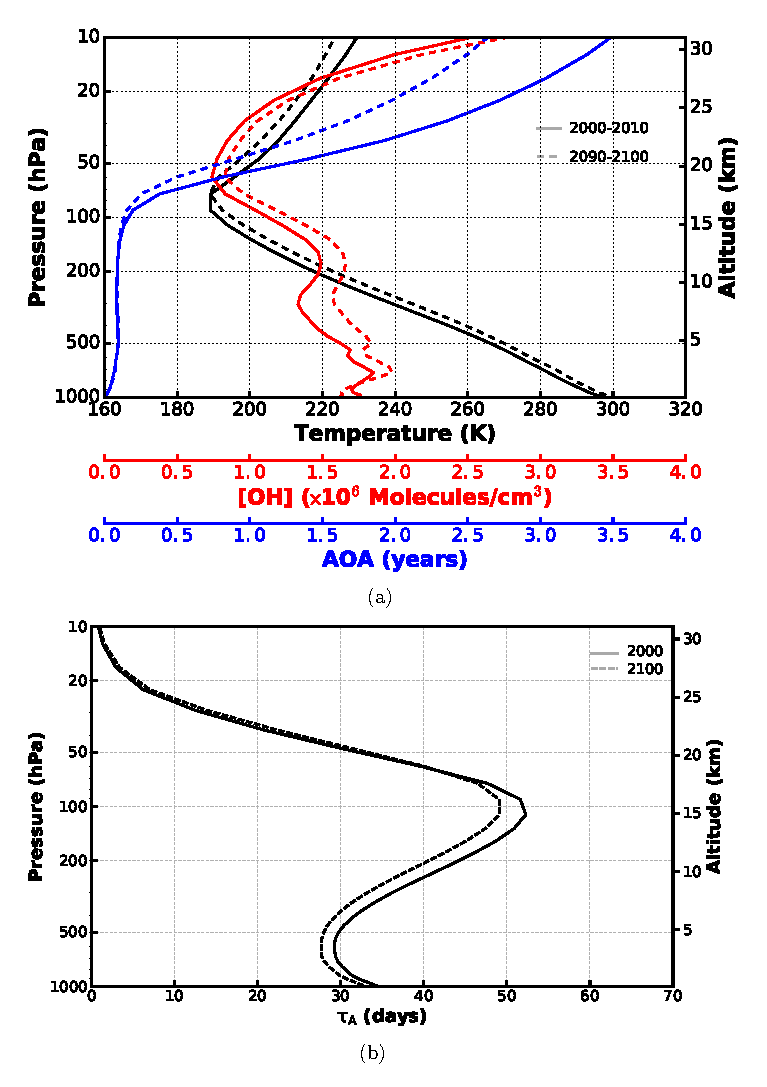
\includegraphics[width=8.3cm]{fig06}
  \caption[]{Tropical average profiles from ESCiMo RC2-base-05 simulation of changing variables in Eq.~(\ref{eq:reaction_rate}) for present day (solid lines) and future (dashed lines).} 
  \label{fig:changing_parameters}
\end{figure}
%
%\begin{figure}[t]
%  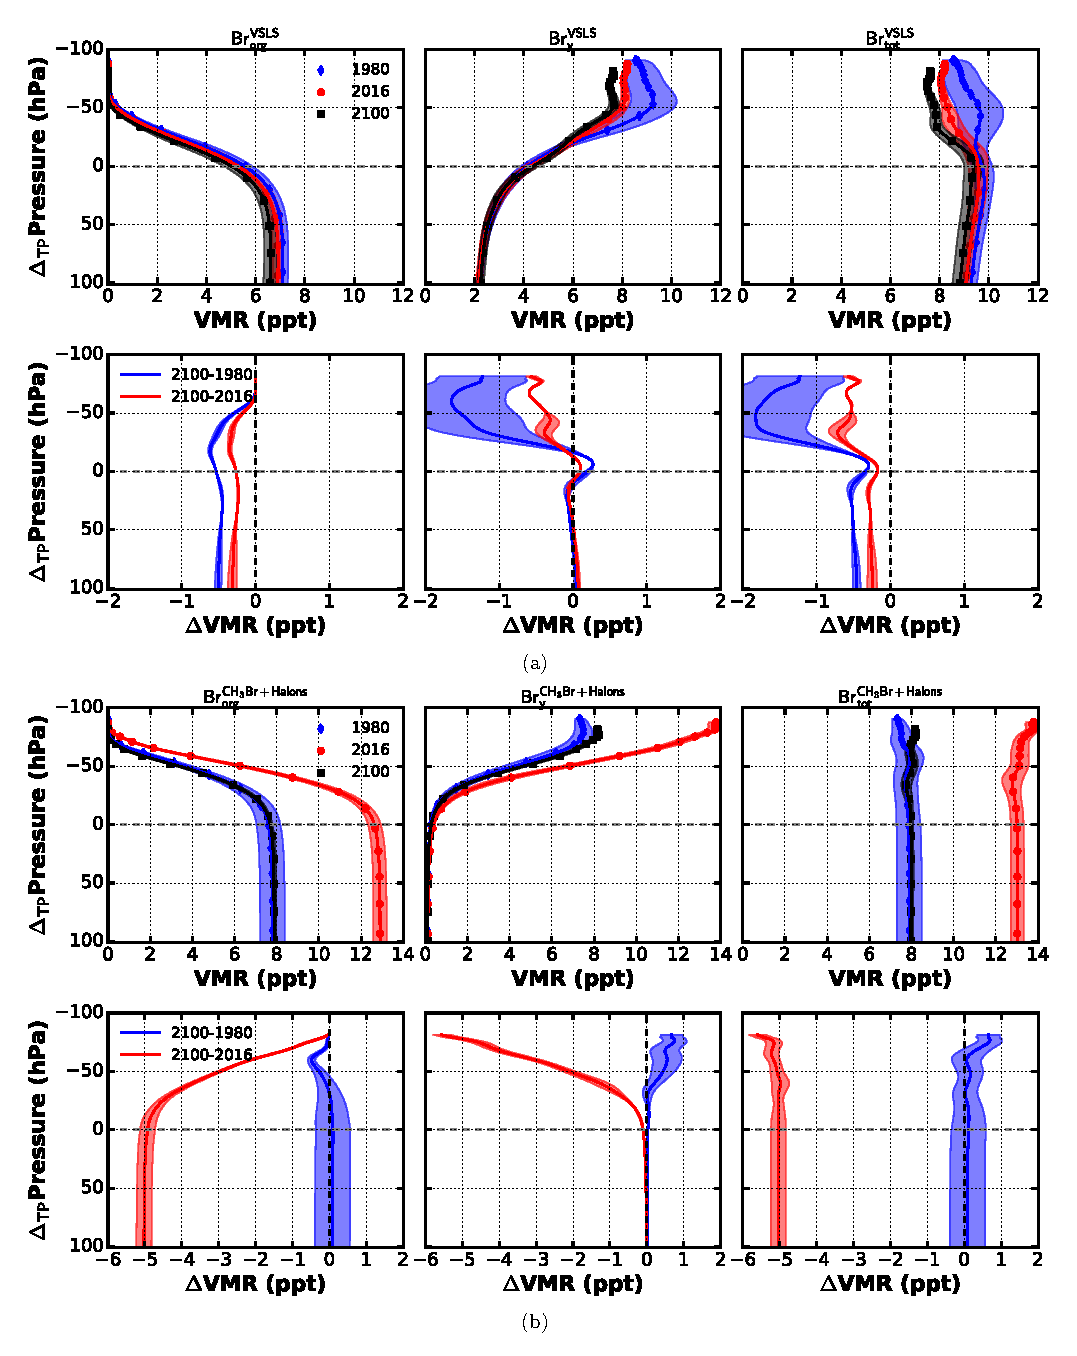
\includegraphics[width=8.3cm]{fig09}
%  \caption[]{Difference in tropospheric AOA between future and present. Tropical average profiles from ESCiMo RC2-base-05 simulation. Monthly means in gray, annual mean in blue.} 
%  \label{fig:delta_aoa_tropics_troposphere}
% \end{figure}
%
%\begin{figure}[t]
%  \centering
%  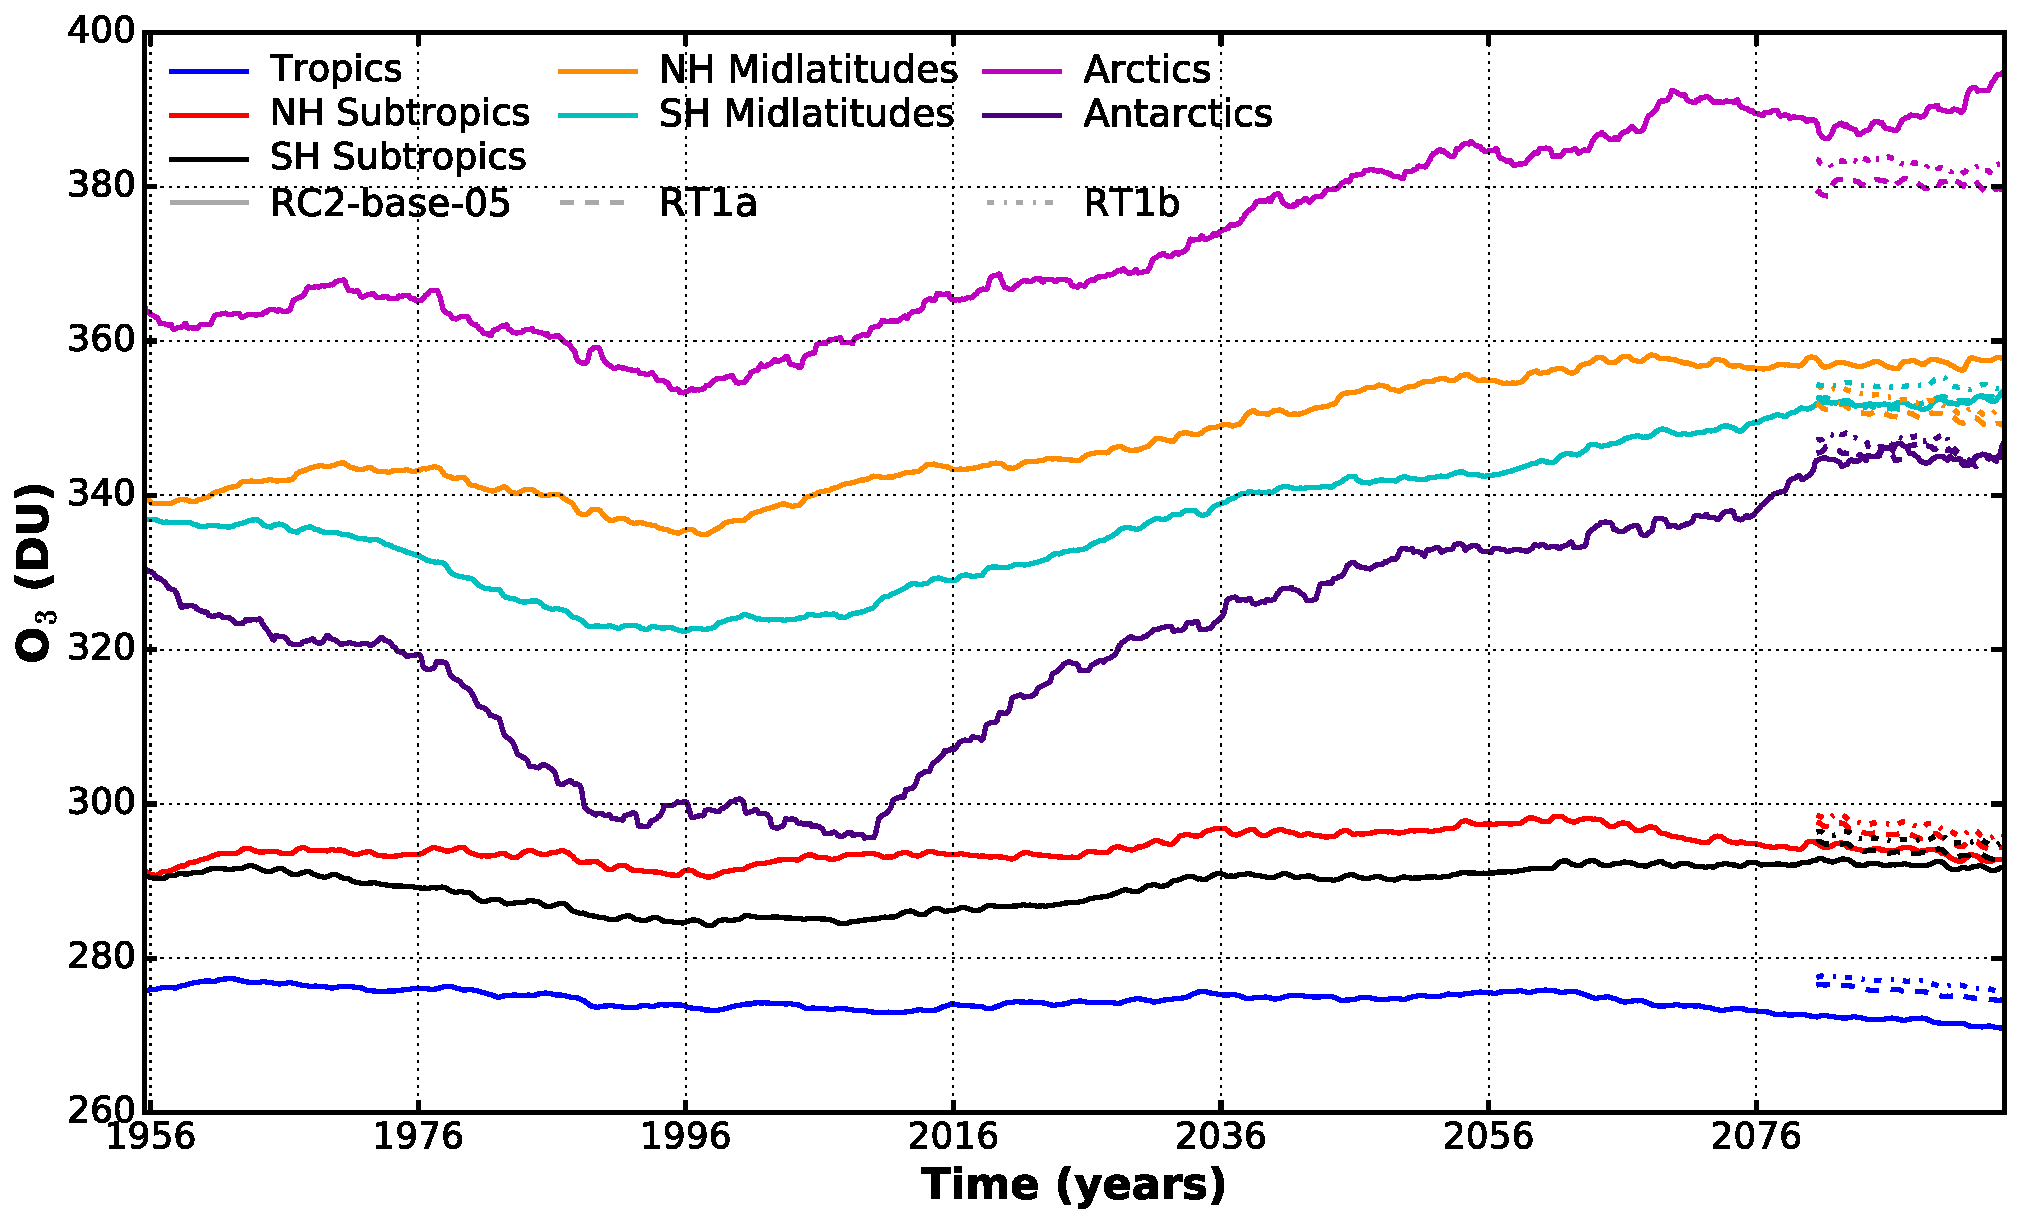
\includegraphics[width=8.3cm]{fig10}
%  \caption[]{Average lifetime of VSLS species $\tau_\mathrm{A}$ due to photolysis for solar zenith angles ranging from 0--90$^\circ$. The average daily lifetime has been inferred from an area weighted mean and accounting for absent photolysis at night times.}
%  \label{fig:vsls_lifetimes}
%\end{figure}
%
\begin{figure}[t]
  \centering
  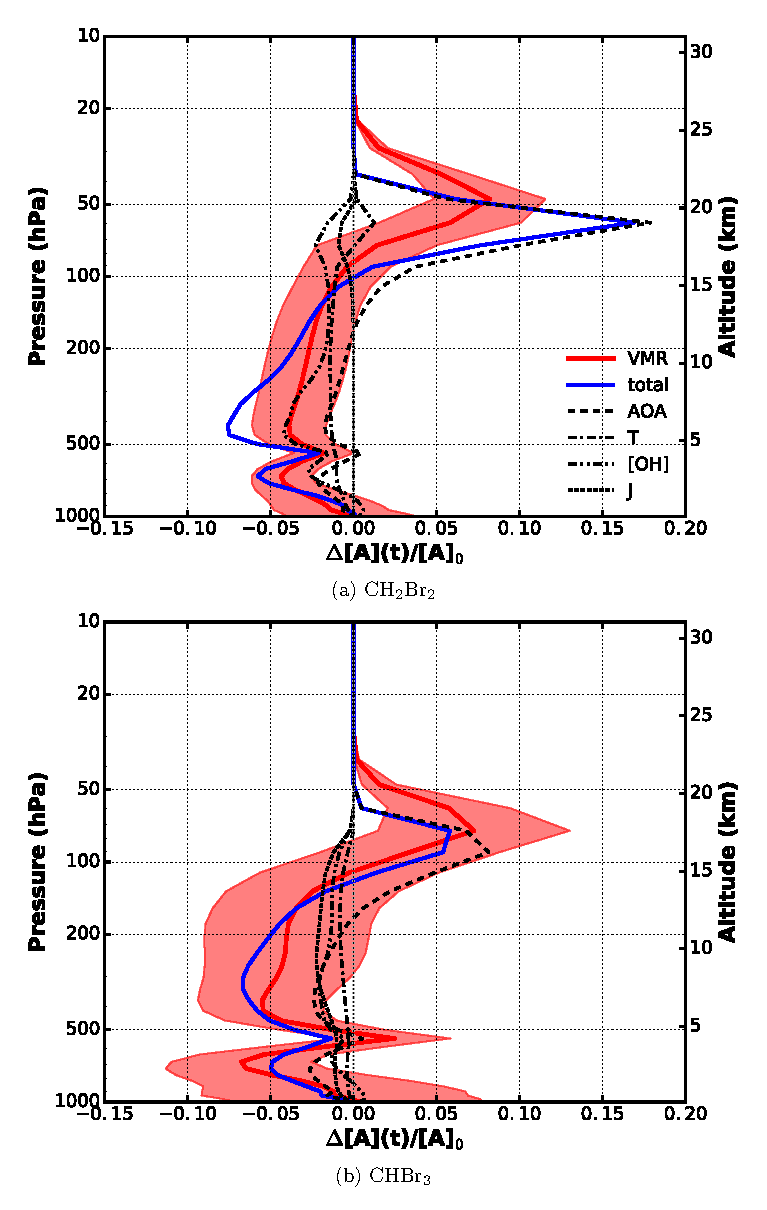
\includegraphics[width=8.3cm]{fig07}
  \caption[]{Relative difference of VSLS vertical profiles for 2000 and 2100. Major influences on lifetime have been separated.Shown are resulting profiles by varying the denoted variables, mean temperature $T$, \chem{OH} concentration [\chem{OH}], photolysis frequency $J$, and age of air~(AOA), in Eq.~(\ref{eq:reaction_rate}) one by one.}
  \label{fig:changing_profiles}
\end{figure}
%
\subsection{Implications of a rising tropopause on VSLS mixing ratio profiles}
\label{subsec:tropopause}
The GHG induced warming of the troposphere and cooling of the stratosphere causes a rise of the tropopause. Model mean tropical tropopause heights from RC2-base-05 have been smoothed using a moving average with a box window size of 11 years. The corresponding standard deviation is displayed as yellow band in Fig.~\ref{fig:tropopause}. A linear regression fit on the smoothed model mean tropical tropopause height yields a rise of $(0.81\pm0.01)$\,\unit{hPa\,decade^{-1}}. This is in accordance with results from ECMWF Re-Analysis data for the past two decades~\citep{QJRMS:Wilcox2012}.  As indicated by~\citet{GRL:Oberlaender2016} regarding the BDC, the upward shift of the tropopause affects the interpretation of vertical profile differences between future and past. An air parcel which would have already entered the stratosphere under present day conditions may be still considered tropospheric in the future. As pointed out earlier, profiles appear shifted by a fraction of distance between two pressure coordinate levels. We perform a spline fit to the averaged profiles and shift them accordingly with respect to the mean tropopause. The fit results have been evaluated within a valid region of $\pm$100\,\unit{hPa} around the tropopause. The results are shown in Fig.~\ref{fig:annual_mean_change_relativ_tp}. Uncertainty bands have been estimated by adding/subtracting one standard deviation from the averaged VMR profiles and computing the corresponding splines. With respect to the mean tropopause, VMR differences show no increase of bromine from VSLS in the lower stratosphere, but rather a slight decrease (Fig.~\ref{fig:annual_mean_change_relativ_tp}a). A small increase of inorganic bromine from VSLS (\chem{Br_y^{VSLS}}) is found in the tropopause region. At about 20\,\unit{hPa}, \chem{Br_y^{VSLS}} is reduced by 1--2\,\unit{ppt} in the future compared to 1980. Overall, a reduction of bromine in the UTLS is found at the end of the 21st century. In Fig.~\ref{fig:annual_mean_change_relativ_tp}b, the amount of bromine from \chem{CH_3Br} and Halons is shown. Except for a slight increase of \chem{Br_{tot}^{CH_3Br+Halons}} in the upper stratosphere between 1980 and 2100 of about 0.7\,\unit{ppt}, there is no increase of bromine from long-lived SG.\\
To summarize, the main reason to the apparent increase of bromine from VSLS above 100\,\unit{hPa} in RC2-base-05 of about 5--10\% is the increase in vertical transport in the tropics.
Although bromine loading from VSLS above 100\,\unit{hPa} is increased at the end of the 21st century, the stratospheric abundance of bromine from VSLS is not increasing but decreasing by about 1--2\,\unit{ppt}, if an upward shift of the tropopause is taken into consideration.
%
\begin{figure}[t]
  \centering
  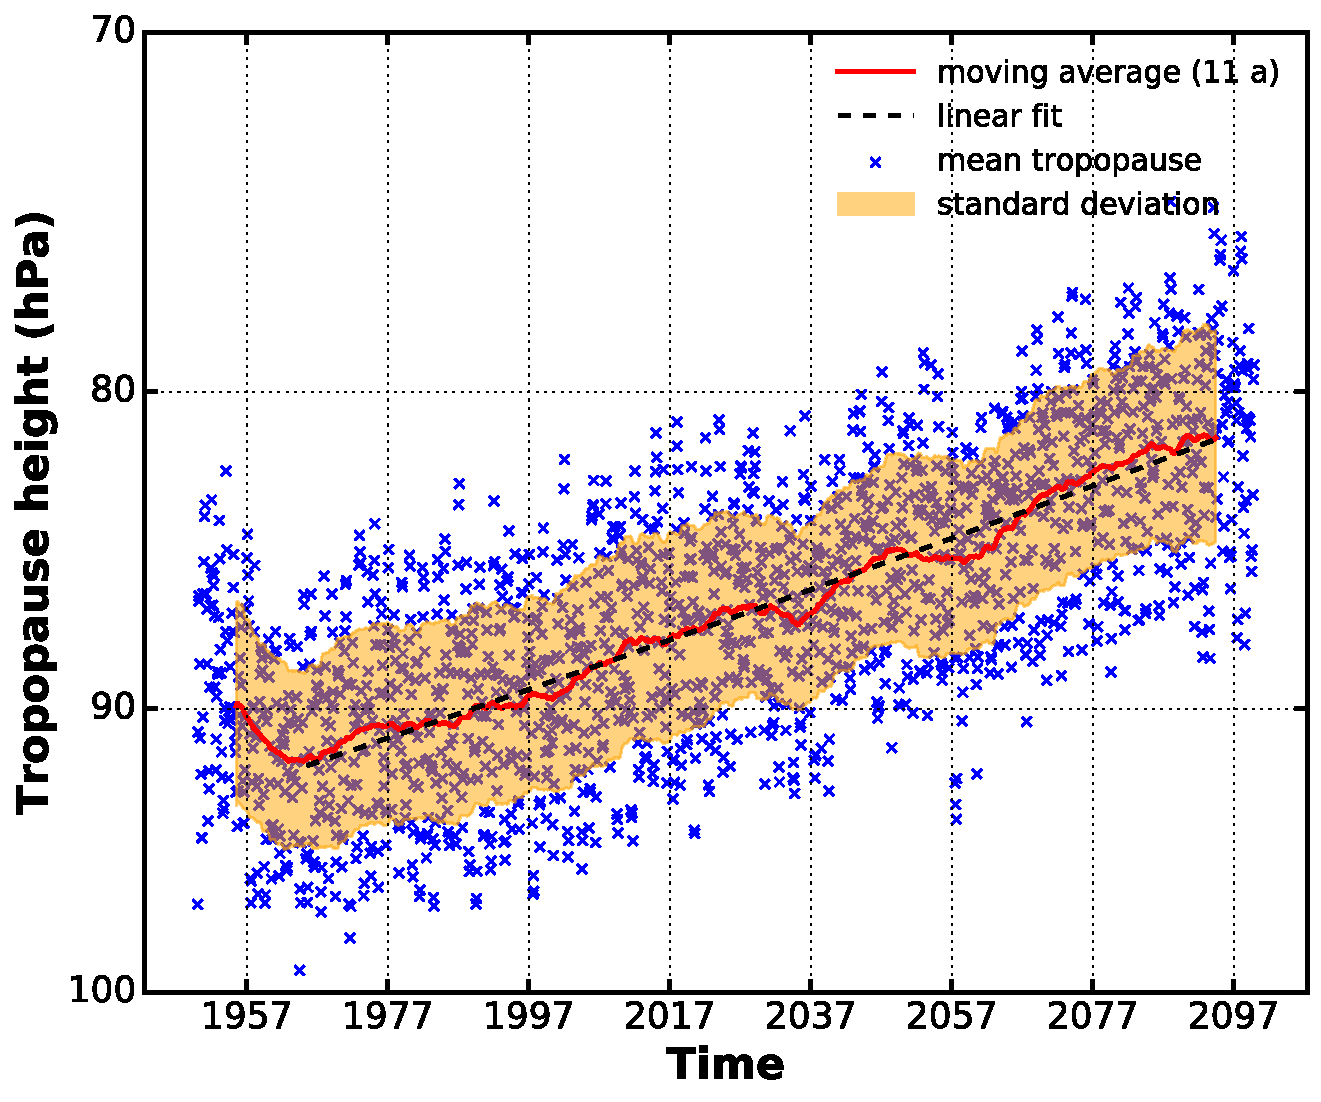
\includegraphics[width=8.3cm]{fig08}
  \caption[]{Model mean tropical tropopause from RC2-base-05 over a time span of 150 years. Tropopause data have been evaluated after the apparent spin-up of about 10 years. A rise of the mean tropical tropopause of $(0.81\pm0.01)$\,\unit{hPa\,decade^{-1}} is found by linear regression.}
  \label{fig:tropopause}
\end{figure}
%
\begin{figure*}[t]
  \centering
  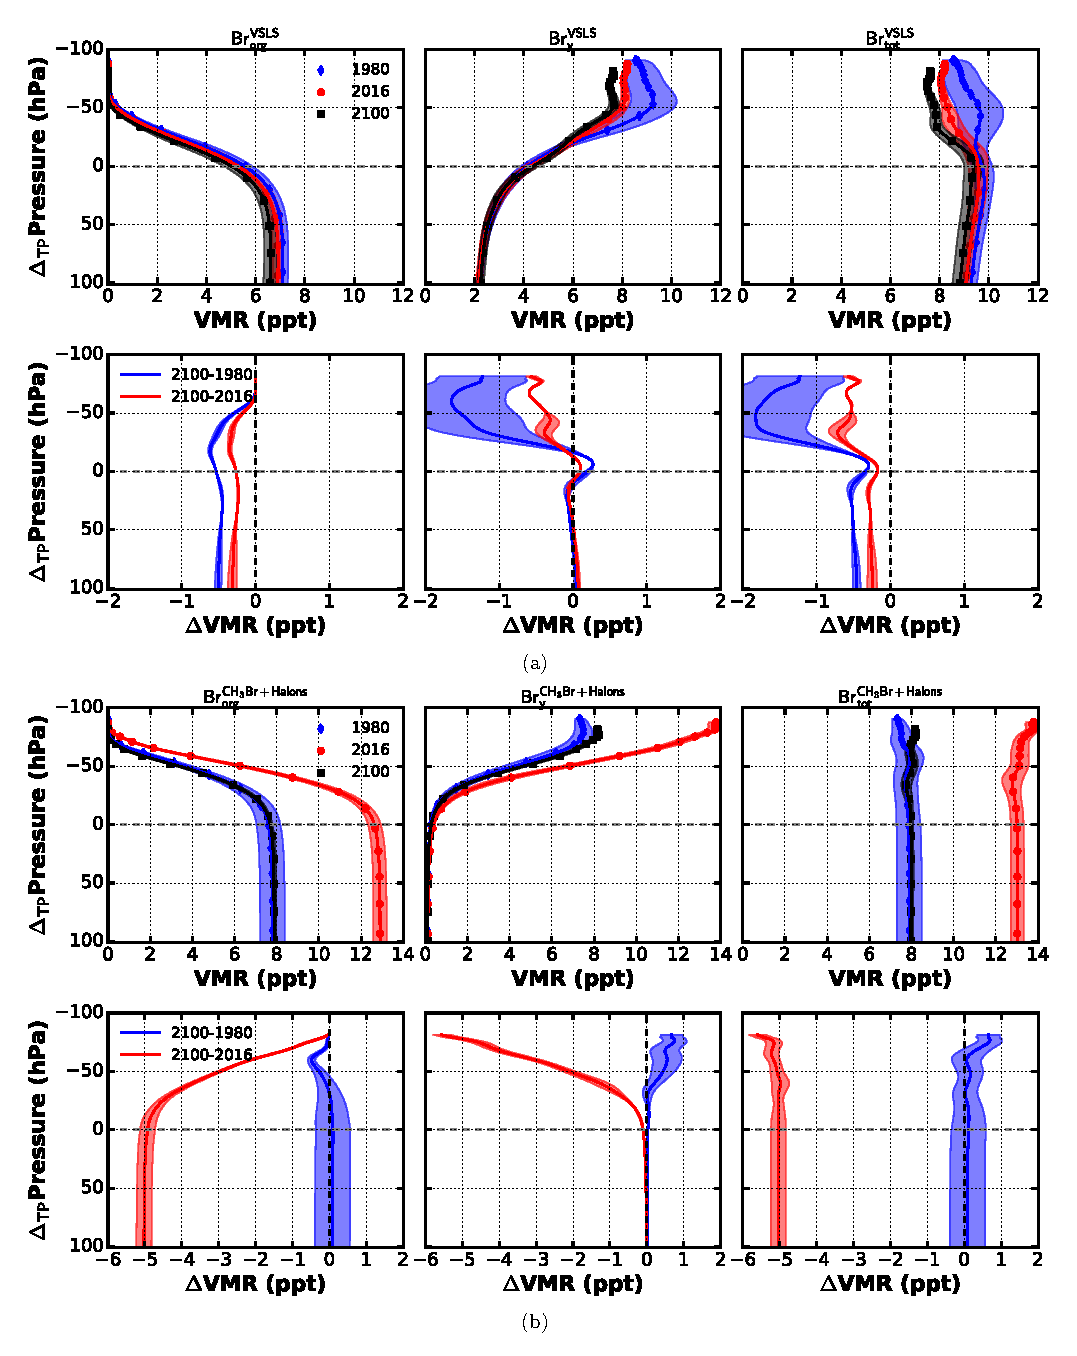
\includegraphics[width=12cm]{fig09} 
  \caption[]{Spline fitted vertical profiles of brominated substances divided into SG (\chem{Br_{org}}), PG (\chem{Br_y}), and SG + PG (\chem{Br_{tot}}) in the tropics (20$^\circ$N--20$^\circ$S) with respect to the mean tropical tropopause. Data from ESCiMo RC2-base-05 simulation~\citep{GMD:Joeckel2016}. Absolute values upper line, difference with respect to 2100 values bottom line. (a) Bromine from VSLS; (b) Bromine from \chem{CH_3Br} and Halons.}
  \label{fig:annual_mean_change_relativ_tp}
\end{figure*}
%
\section{Implications on ozone depletion}
\label{sec:ozone_depletion}
In this section, the influence of brominated very short-lived source gases on ozone depletion will be studied based on RT1a and RT1b. For a thorough discussion of future trends, the 25 year data set is too short. Results from RC2-base-05 cannot be compared to RT1a/RT1b directly, because of significant differences in ozone distribution and amount between the differing vertical resolutions (L47MA and L90MA) of the model. This issue has been already reported by~\citet{GMD:Joeckel2016}.\\ 
Zonally averaged data of total column ozone have been smoothed using a moving average algorithm with box window size of 11 years (Fig.~\ref{fig:Zonal_Total_Ozone}). In general, ozone trends at the end of the century are roughly the same for both resolutions. The actual amount of ozone differs, with L90 showing more ozone except for the northern hemisphere polar region and mid-latitudes. In the Arctic RT1a/RT1b even indicate, in contrast to RC2-base-05, slightly decreasing total column ozone. In case of RT1a/RT1b, this might be partially caused by interactive aerosol and accordingly added oceanic COS source. This bias in total column ozone between the vertical resolutions is larger than the difference between RT1a and RT1b.\\
%
For estimating the effect of brominated VSLS on ozone depletion, the difference in zonally averaged ozone of RT1a and RT1b has been computed. A period of 20 years (2080--2100) has been used accounting for an estimated model spin-up of five years in the beginning. In Fig.~\ref{fig:zonal_mean_ozone}, the relative difference ($\mathrm{(RT1a-RT1b)}/\mathrm{RT1a}\cdot100$) is shown as contour plot. Dashed lines indicate a decrease of ozone in the simulation with VSLS turned on (RT1a) compared to the one with VSLS turned off (RT1b), while solid lines indicate an increase. The average tropopause is shown as red line. VSLS cause a tropospheric ozone reduction in the order of 1--2\%, mainly at high latitudes. The UTLS region in the tropics is most affected, there VSLS cause a decrease of ozone of about 3\%. Increasing amounts of ozone ($\sim$1\%) are found in the Antarctic middle and upper stratosphere, but these are mainly not significant. Significance has been estimated as divergence from zero in units of standard error of mean. It is indicated by shades of blue. High latitude decrease of ozone in the troposphere and tropical UTLS is rendered significant.\\
%
\citet{GRL:Sinnhuber2015} have shown a reduction of ozone due to VSLS in the TTL region in the order of 6\% during the period 1970--1982 with significantly less stratospheric chlorine compared to the later period 1983--2005 (7\%), while ~\citet[Supplement][Fig.~S3]{NGS:Hossaini2015} show a change of total ozone column due to VSLS (on/off scenario) of the order of 1--3\% in pre-industrial conditions. Given that scenario five of~\citet{JGR:Warwick2006} has about double the amount of VSLS compared to RT1a and chlorine abundance in the stratosphere will drop to 1970 values by the end of the 21st century~\citep[see][Chap. 12]{IPCC2013}, our results are in good agreement with these previous analysis. 
%
\begin{figure}[t]
  \centering
  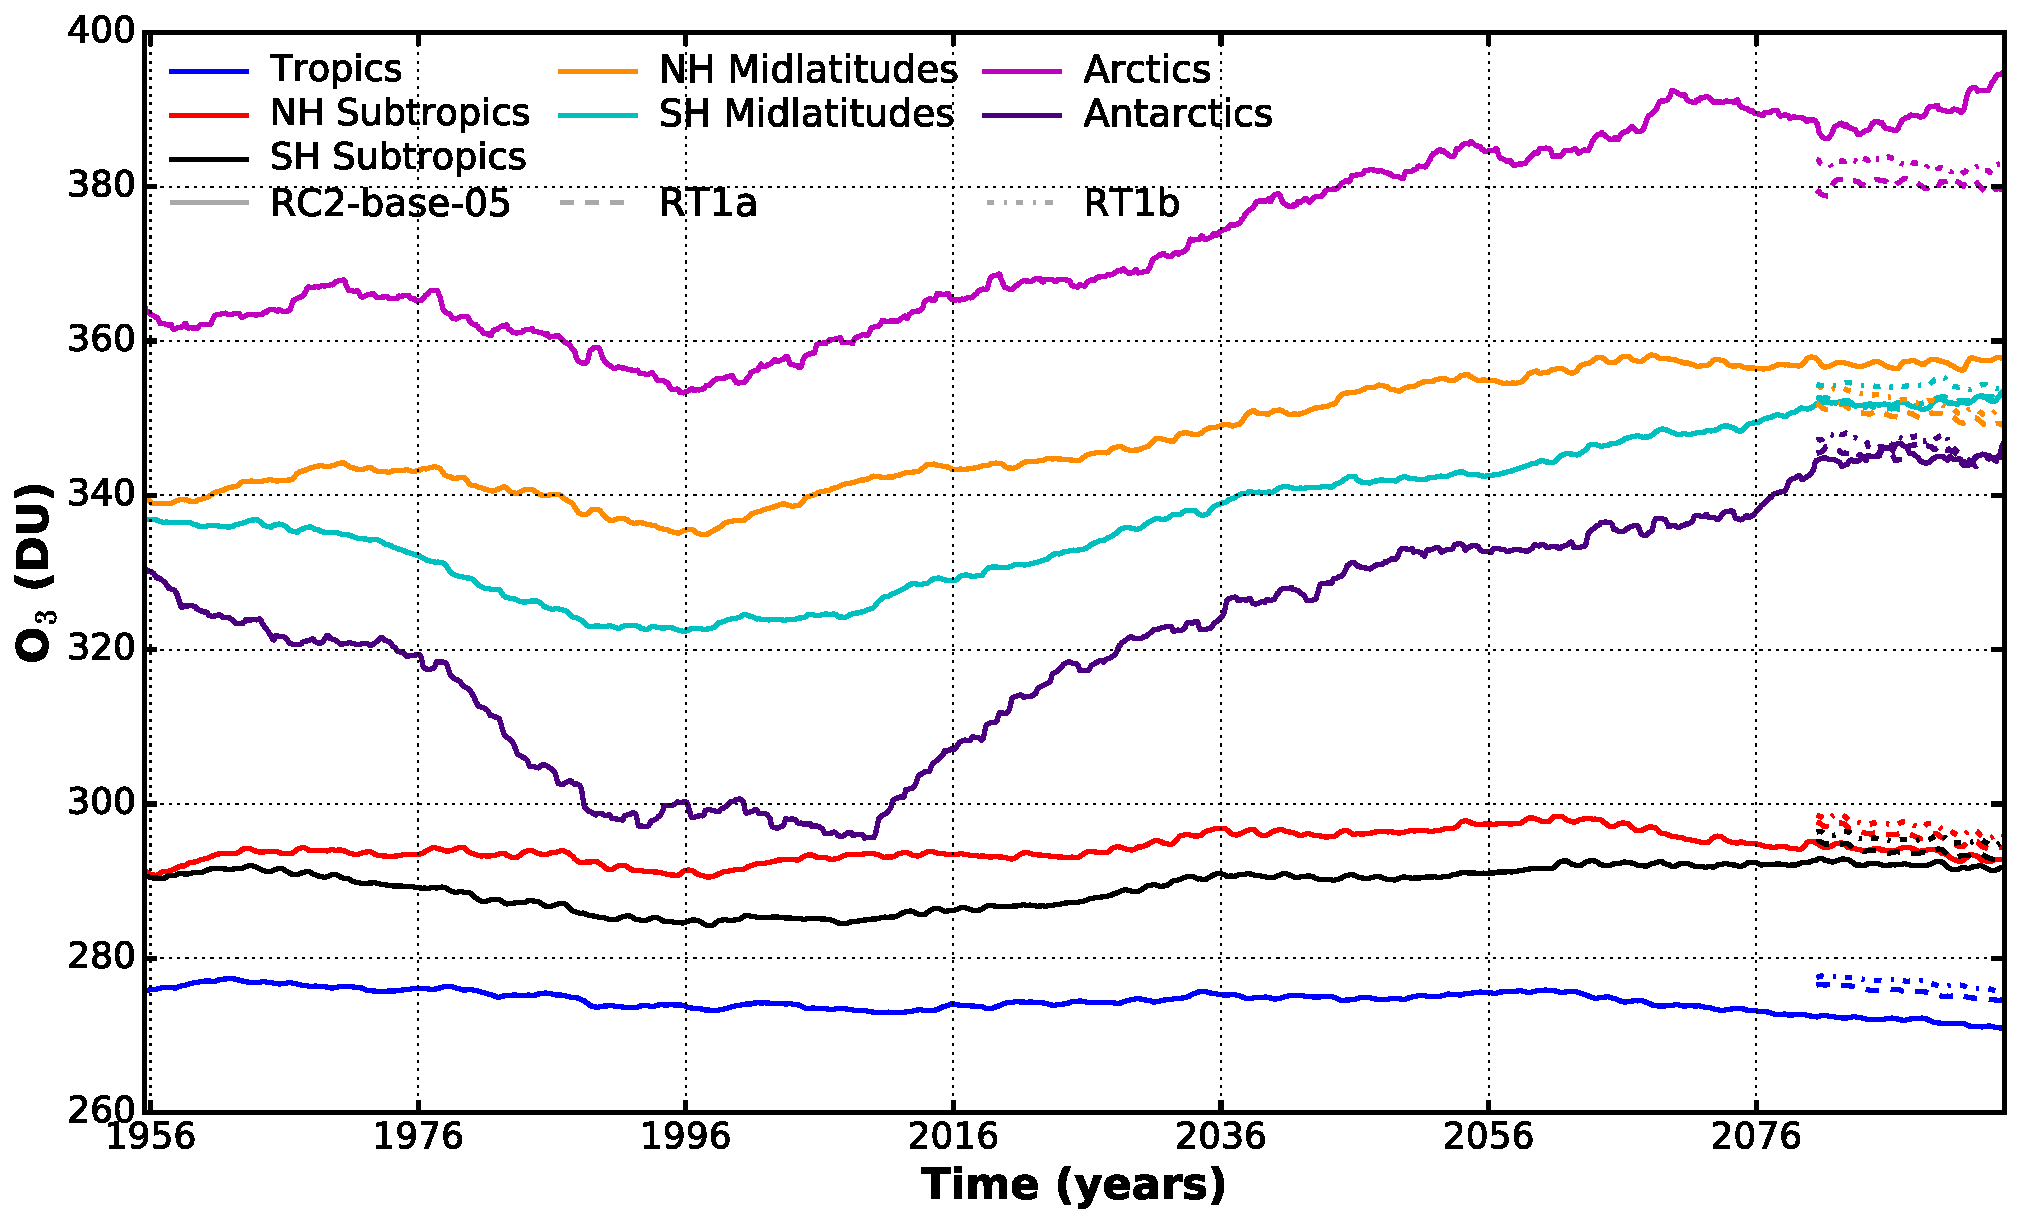
\includegraphics[width=8.3cm]{fig10}
  \caption{Zonal mean ozone trend from RC2-base-05 (1950--2100) and RT1a/RT1b (2080--2100). Smoothed with moving average box window 11 years.}
  \label{fig:Zonal_Total_Ozone}
\end{figure}
%
\begin{figure*}[t]
  \centering
  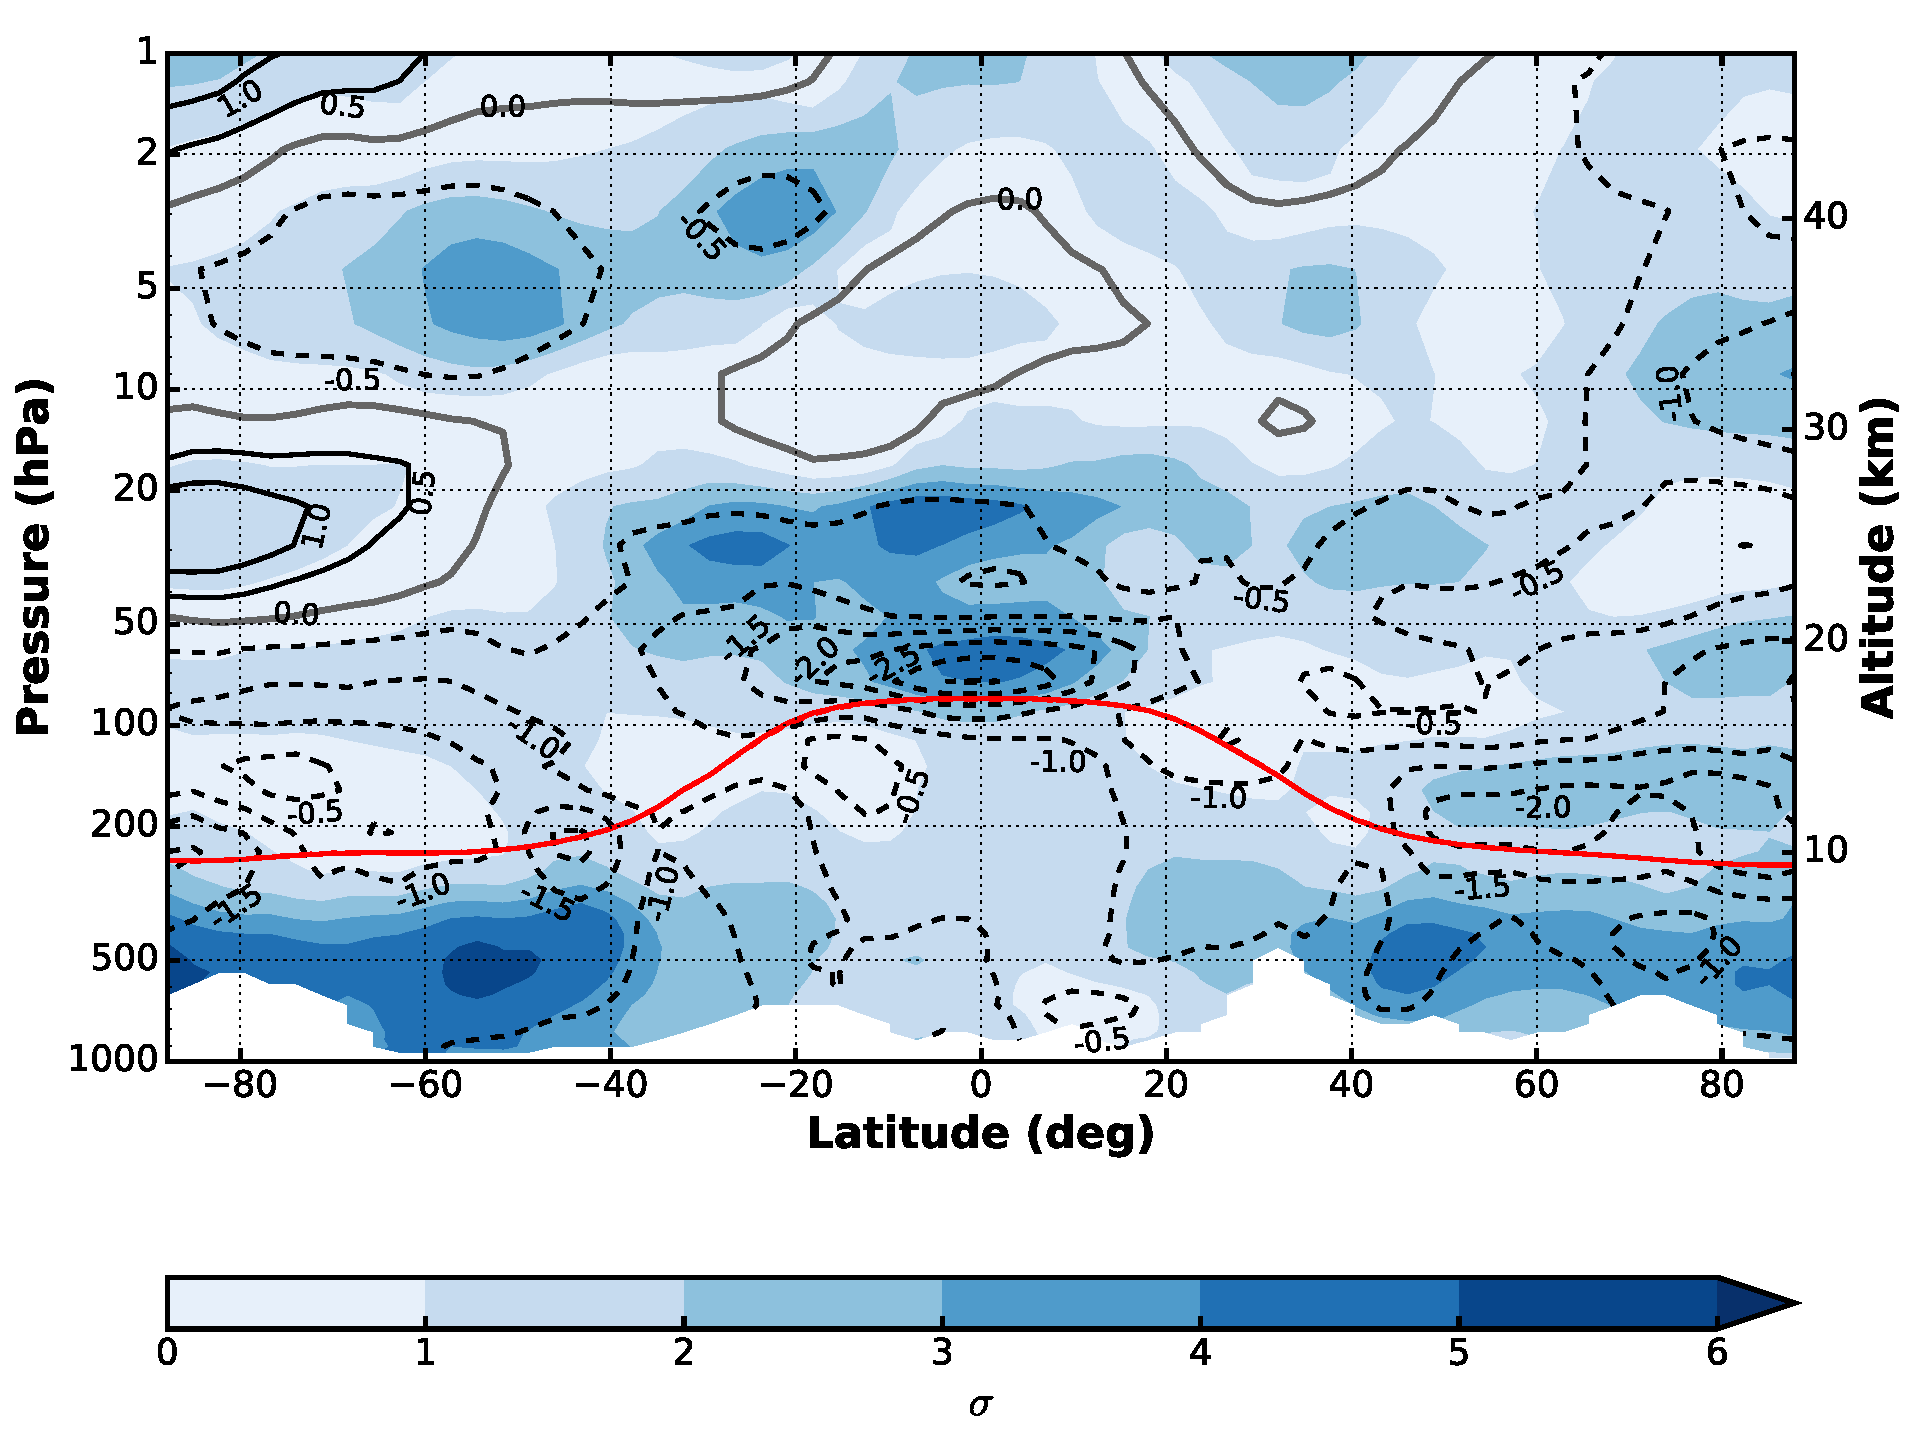
\includegraphics[width=12cm]{fig11}
  \caption{Ozone reduction due to VSLS. Medium-term full-chemistry future simulation with and without VSLS. Zonal mean profile of decadal mean difference in percent ($\mathrm{(RT1a-RT1b)/RT1a\cdot100}$). Dashed lines indicate a decrease of ozone in the simulation with VSLS turned on (RT1a) compared to the one with VSLS turned off (RT1b). The average tropopause is shown as red line. Significance is indicated by blue shaded areas. The significance is estimated as manifold of difference from zero in units of standard error of mean difference.}
  \label{fig:zonal_mean_ozone}
\end{figure*}
%
\conclusions  %% \conclusions[modified heading if necessary]
\label{sec:conclusion}
We have investigated long-term changes in emission and transport of brominated VSLS under a changing climate (RCP6.0). Under the implicit assumption of constant concentrations of VSLS in the ocean waters, over a time-span of 120 years, we have found an enhancement of zonally averaged fluxes of \chem{CH_2Br_2} and \chem{CHBr_3} in the order of 10\% between present day and the end of the 21st century. A strong increase of flux (up to 55\% in \chem{CH_2Br_2} and 25\% in \chem{CHBr_3}) has been found in the northern hemisphere polar region. There, the retreat of sea ice is playing a key role. Exposing almost the entire polar ocean in August--September by the end of the 21st century, sea ice does not longer act as a lid to ocean--atmosphere fluxes of VSLS. Sea ice itself has not been considered a source of VSLS in our simulations. The subsequent increase of organic bromine in the UTLS is of the same order of magnitude (8--10\%).\\
%
Since ocean--atmosphere fluxes are sensitive to the abundance of VSLS in the atmosphere, an increased dissociation of VSLS in the lowermost troposphere, e.g., due to increasing \chem{OH} concentrations in the RCP6.0 scenario, reduces the atmospheric concentration and therefore increases the flux from the ocean to the atmosphere without necessarily increasing the actual amount which is transported to the stratosphere.\\
%
Assuming a constant, prescribed flux of VSLS over the course of 150 years, we have developed a simple, analytic ansatz to disentangled various factors affecting the future abundance of bromine from VSLS in the atmosphere. All occurring future changes in temperature, [\chem{OH}], AOA, and photolysis frequency decrease the VMR of VSLS in the troposphere (in total $\sim$5--10\%). In case of \chem{CHBr_3}, all factors listed are of the same order of magnitude. The tropospheric decrease of \chem{CH_2Br_2} VMR is mainly driven by increasing [\chem{OH}]. In the UTLS, the impact of rejuvenating AOA dominates, inflicting an increase in VSLS VMR in the order of 5--10\%. In general, the features of the actual difference profiles are well reproduced by our ansatz. The effect of AOA on \chem{CH_2Br_2} is, however, slightly overestimated.\\
%
Due to the rise of the tropical tropopause by 0.81\,\unit{hPa\,decade^{-1}}, air which at present is considered stratospheric will be still tropospheric in the future. If taken into account by shifting VSLS VMR profiles with respect to the mean model tropopause height, the total amount of bromine in the tropical UTLS is decreasing by roughly 2\,\unit{ppt}. Overall, the amount of bromine in the UTLS is decreasing in this future scenario.\\
%
The impact of enhanced fluxes of brominated VSLS on future ozone abundance has been evaluated by comparing two experiments of which one has no VSLS emission and the other interactively computed fluxes from constant ocean concentrations of VSLS. We have found a significant reduction of ozone in the tropical UTLS of about 3\%. In the troposphere the largest significant decrease of ozone amounts to 1--2\%. Thus, bromine from VSLS may not act as a major source to future stratospheric ozone depletion.
%
While interactive emissions from constant ocean concentrations and aerosol formation have been taken into consideration, the actual climate change inflicted change in the production of VSLS by macroalgae in the ocean remains an open question. Whether the found increase of ocean--atmosphere fluxes of VSLS and a future decrease of VSLS in the troposphere will cancel out or overcompensate would need further simulation studies.
%
%\section{Code availability}
%TEXT
\section{Data availability}
The Modular Earth Submodel System (MESSy) is continuously further developed and applied by a consortium of institutions. The usage of MESSy and access to the source code is licensed to all affiliates of institutions, which are members of the MESSy Consortium. Institutions can become a member of the MESSy Consortium by signing the MESSy Memorandum of Understanding. More information can be found on the MESSy Consortium Web-site (\url{http://www.messy-interface.org}).\\
The data of the ESCiMo simulations will be made available in the Climate and Environmental Retrieval and Archive (CERA) database at the German Climate Computing Centre (DKRZ; \url{http://cera-www.dkrz.de/WDCC/ui/Index.jsp}). The corresponding digital object identifiers (doi) will be published on the MESSy consortium web-page (\url{http://www.messy-interface.org}). A subset of the data of those simulations covering consistently the requested time periods (1960--2010 for RC1, and 1960--2099 for RC2) will be submitted to the BADC database for the CCMI project.\\
Data from ROMIC--THREAT associated simulations (RT1a, RT1b) and simplified chemistry (SC\_free, SC\_nudged) will be made available on request.
%\appendix
%\section{}    %% Appendix A

%\subsection{}     %% Appendix A1, A2, etc.

%\appendixfigures  %% needs to be added in front of appendix figures in one-column style (\documentclass[acp, manuscript]{copernicus})

%\appendixtables   %% needs to be added in front of appendix tables in one-column style (\documentclass[acp, manuscript]{copernicus})

\authorcontribution{S. Falk performed most of the analyses and wrote the paper. B.-M. Sinnhuber conceived this study and provided advice. G. Krysztofiak developed and performed the simplified chemistry simulations as well as part of the corresponding data analysis in Sec.~\ref{sec:emission_trends}. S.~T. Lennatz provided advise on the ocean--atmosphere gas exchange. P. J\"{o}ckel provided advice as project leader of the ESCiMo consortial project and coordinator of overall EMAC model development; preparation of the ESCiMo model setups and realization of the ESCiMo simulations of ESCiMo consortium, with VSLS boundary conditions and implementation of the online \chem{Br} budget diagnostics for EMAC prepared by P. Graf. All coauthors contributed to the discussion of the results.}

\competinginterests{The authors declare that they have no conflict of interest.}

%\disclaimer{TEXT}

\begin{acknowledgements}
Parts of this work were supported by the Deutsche Forschungsgemeinschaft (DFG) through the research unit 'SHARP' (SI1044/1-2), the German Bundesministerium f\"{u}r Bildung und Forschung (BMBF) through the project 'ROMIC-THREAT' (01GL1217B), the European Union through the Horizon 2020 project 'GAIA-CLIM', and by the Helmholtz Association through its research program 'ATMO'.\\
The CNRM data were produced in the framework of the CCMI project, with support of M\'{e}t\'{e}o--France. We particularly acknowledge the support of M. Michou and D. Saint--Martin and of the entire team in charge of the CNRM/CERFACS climate model.\\
NOAA Optimum Interpolation~(OI)~V2 fields were provided by the National Centers for Environmental Prediction/National Weather Service/NOAA/U.S. Department of Commerce, and National Climatic Data Center/NESDIS/NOAA/U.S. Department of Commerce research Data Archive at the National Center for Atmospheric Research, Computational and Information Systems Laboratory. \url{http://rda.ucar.edu/datasets/ds277.0/}. Accessed 06 January 2016).\\
The ESCiMo (Earth System Chemistry integrated Modelling) model simulations have been performed at the German Climate Computing Centre~(DKRZ) through support from the BMBF. DKRZ and its scientific steering committee are gratefully acknowledged for providing the HPC and data archiving resources for this consortial project.\\
EMAC simulations RT1a/1b have been performed at Steinbuch Center for Computing at KIT. Thanks to Stefan Versick and Oliver Kirner for their technical support.\\
Special thanks to C. Br\"{u}hl (MPI-Mainz) for his help in implementing additional sulfur reactions and usage of \texttt{gmxe} in context of the ROMIC--THREAT simulations.\\
S. Lennartz likes to thank B. Quack, C. Marandino, S. Tegtmeier (all Helmholtz-Centre for Ocean Research Kiel), and K. Kr\"{u}ger (University of Oslo) for their support.
\end{acknowledgements}

%% REFERENCES
%% Since the Copernicus LaTeX package includes the BibTeX style file copernicus.bst,
%% authors experienced with BibTeX only have to include the following two lines:
%%
\bibliographystyle{copernicus}
\bibliography{vsls_emissions}
%%
%% URLs and DOIs can be entered in your BibTeX file as:
%%
%% URL = {http://www.xyz.org/~jones/idx_g.htm}
%% DOI = {10.5194/xyz}

%% LITERATURE CITATIONS
%%
%% command                        & example result
%% \citet{jones90}|               & Jones et al. (1990)
%% \citep{jones90}|               & (Jones et al., 1990)
%% \citep{jones90,jones93}|       & (Jones et al., 1990, 1993)
%% \citep[p.~32]{jones90}|        & (Jones et al., 1990, p.~32)
%% \citep[e.g.,][]{jones90}|      & (e.g., Jones et al., 1990)
%% \citep[e.g.,][p.~32]{jones90}| & (e.g., Jones et al., 1990, p.~32)
%% \citeauthor{jones90}|          & Jones et al.
%% \citeyear{jones90}|            & 1990

%% FIGURES

%% We suggest to put the figures in the correct order and placement within the text. This aids readability.
%% When figures and tables are placed at the end of the MS (article in one-column style), please add \clearpage
%% between bibliography and first table and/or figure as well as between each table and/or figure.

%% ONE-COLUMN FIGURES
%%f
%\begin{figure}[t]
%\includegraphics[width=8.3cm]{FILE NAME}
%\caption{TEXT}
%\end{figure}
%
%%% TWO-COLUMN FIGURES
%
%%f
%\begin{figure*}[t]
%\includegraphics[width=12cm]{FILE NAME}
%\caption{TEXT}
%\end{figure*}
%
%
%%% TABLES
%%%
%%% The different columns must be seperated with a & command and should
%%% end with \\ to identify the column brake.
%
%%% ONE-COLUMN TABLE
%
%%t
%\begin{table}[t]
%\caption{TEXT}
%\begin{tabular}{column = lcr}
%\tophline
%
%\middlehline
%
%\bottomhline
%\end{tabular}
%\belowtable{} % Table Footnotes
%\end{table}
%
%%% TWO-COLUMN TABLE
%
%%t
%\begin{table*}[t]
%\caption{TEXT}
%\begin{tabular}{column = lcr}
%\tophline
%
%\middlehline
%
%\bottomhline
%\end{tabular}
%\belowtable{} % Table Footnotes
%\end{table*}
%
%
%%% MATHEMATICAL EXPRESSIONS
%
%%% All papers typeset by Copernicus Publications follow the math typesetting regulations
%%% given by the IUPAC Green Book (IUPAC: Quantities, Units and Symbols in Physical Chemistry,
%%% 2nd Edn., Blackwell Science, available at: http://old.iupac.org/publications/books/gbook/green_book_2ed.pdf, 1993).
%%%
%%% Physical quantities/variables are typeset in italic font (t for time, T for Temperature)
%%% Indices which are not defined are typeset in italic font (x, y, z, a, b, c)
%%% Items/objects which are defined are typeset in roman font (Car A, Car B)
%%% Descriptions/specifications which are defined by itself are typeset in roman font (abs, rel, ref, tot, net, ice)
%%% Abbreviations from 2 letters are typeset in roman font (RH, LAI)
%%% Vectors are identified in bold italic font using \vec{x}
%%% Matrices are identified in bold roman font
%%% Multiplication signs are typeset using the LaTeX commands \times (for vector products, grids, and exponential notations) or \cdot
%%% The character * should not be applied as mutliplication sign
%
%
%%% EQUATIONS
%
%%% Single-row equation
%
%\begin{equation}
%
%\end{equation}
%
%%% Multiline equation
%
%\begin{align}
%& 3 + 5 = 8\\
%& 3 + 5 = 8\\
%& 3 + 5 = 8
%\end{align}
%
%
%%% MATRICES
%
%\begin{matrix}
%x & y & z\\
%x & y & z\\
%x & y & z\\
%\end{matrix}
%
%
%%% ALGORITHM
%
%\begin{algorithm}
%\caption{�}
%\label{a1}
%\begin{algorithmic}
%�
%\end{algorithmic}
%\end{algorithm}
%
%
%%% CHEMICAL FORMULAS AND REACTIONS
%
%%% For formulas embedded in the text, please use \chem{}
%
%%% The reaction environment creates labels including the letter R, i.e. (R1), (R2), etc.
%
%\begin{reaction}
%%% \rightarrow should be used for normal (one-way) chemical reactions
%%% \rightleftharpoons should be used for equilibria
%%% \leftrightarrow should be used for resonance structures
%\end{reaction}
%
%
%%% PHYSICAL UNITS
%%%
%%% Please use \unit{} and apply the exponential notation


\end{document}
